%%%%%%%% ICML 2026 EXAMPLE LATEX SUBMISSION FILE %%%%%%%%%%%%%%%%%

\documentclass{article}

% Recommended, but optional, packages for figures and better typesetting:
\usepackage{microtype}
\usepackage{graphicx}
\usepackage{subcaption}
\usepackage{booktabs} % for professional tables

% hyperref makes hyperlinks in the resulting PDF.
% If your build breaks (sometimes temporarily if a hyperlink spans a page)
% please comment out the following usepackage line and replace
% \usepackage{icml2026} with \usepackage[nohyperref]{icml2026} above.
\usepackage{hyperref}


% Attempt to make hyperref and algorithmic work together better:
\newcommand{\theHalgorithm}{\arabic{algorithm}}

% Use the following line for the initial blind version submitted for review:
%\usepackage{icml2026}

% For preprint, use
 \usepackage[preprint]{icml2026}

% If accepted, instead use the following line for the camera-ready submission:
% \usepackage[accepted]{icml2026}

\usepackage{amsmath}
\usepackage{amssymb}
\usepackage{mathtools}
\usepackage{amsthm, thm-restate}
\usepackage{algorithm}
\usepackage{comment}
%\usepackage{algpseudocode}

\usepackage{enumitem}

\usepackage{xspace}
\makeatletter
\DeclareRobustCommand\onedot{\futurelet\@let@token\@onedot}
\def\@onedot{\ifx\@let@token.\else.\null\fi\xspace}

\def\iid{{i.i.d}\onedot}
\def\eg{{e.g}\onedot} \def\Eg{{E.g}\onedot}
\def\ie{{i.e}\onedot} \def\Ie{{I.e}\onedot}
\def\cf{{c.f}\onedot} \def\Cf{{C.f}\onedot}
\def\etc{{etc}\onedot} \def\vs{{vs}\onedot}
\def\wrt{w.r.t\onedot} \def\dof{d.o.f\onedot}
\def\etal{\emph{et al}\onedot}
\makeatother

% if you use cleveref..
\usepackage[capitalize,noabbrev]{cleveref}

%%%%%%%%%%%%%%%%%%%%%%%%%%%%%%%%
% THEOREMS
%%%%%%%%%%%%%%%%%%%%%%%%%%%%%%%%
\theoremstyle{plain}
\newtheorem{theorem}{Theorem} % disable per-section theorem numbering
%\newtheorem{theorem}{Theorem}[section]
\newtheorem{proposition}[theorem]{Proposition}
\newtheorem{lemma}[theorem]{Lemma}
\newtheorem{corollary}[theorem]{Corollary}
\theoremstyle{definition}
%\newtheorem{definition}[theorem]{Definition}
\newtheorem{definition}{Definition}   % disable definition to follow thereom numbering
\newtheorem{assumption}[theorem]{Assumption}
\theoremstyle{remark}
\newtheorem{remark}[theorem]{Remark}

\DeclareMathOperator\supp{supp}
\newcommand{\method}{DP-$\lambda$CGD\xspace}

% Todonotes is useful during development; simply uncomment the next line
%    and comment out the line below the next line to turn off comments
%\usepackage[disable,textsize=tiny]{todonotes}
\usepackage[textsize=tiny]{todonotes}

% The \icmltitle you define below is probably too long as a header.
% Therefore, a short form for the running title is supplied here:
\icmltitlerunning{\method: Efficient Noise Correlation for Differentially Private Model Training}

\begin{document}
%\addtolength{\dbltextfloatsep}{-2pt}
%\addtolength{\dblfloatsep}{-2pt}
%\addtolength{\intextsep}{-2pt}
%\addtolength{\abovedisplayskip}{-.15\baselineskip}
%\addtolength{\belowdisplayskip}{-.15\baselineskip}


\twocolumn[
  \icmltitle{\method: Efficient Noise Correlation for 
  Differentially Private Model Training}

  % It is OKAY to include author information, even for blind submissions: the
  % style file will automatically remove it for you unless you've provided
  % the [accepted] option to the icml2026 package.

  % List of affiliations: The first argument should be a (short) identifier you
  % will use later to specify author affiliations Academic affiliations
  % should list Department, University, City, Region, Country Industry
  % affiliations should list Company, City, Region, Country

  % You can specify symbols, otherwise they are numbered in order. Ideally, you
  % should not use this facility. Affiliations will be numbered in order of
  % appearance and this is the preferred way.
  \icmlsetsymbol{equal}{*}

  \begin{icmlauthorlist}
    \icmlauthor{Nikita P. Kalinin}{yyy}
    \icmlauthor{Ryan McKenna}{comp}
    \icmlauthor{Rasmus Pagh}{xxx}
    \icmlauthor{Christoph Lampert}{yyy}
  \end{icmlauthorlist}

  \icmlaffiliation{yyy}{Institute of Science and Technology Austria, Klosterneuburg, Austria}
  \icmlaffiliation{comp}{Google, Seattle, US}
  \icmlaffiliation{xxx}{University of Copenhagen, Copenhagen, Denmark}

  \icmlcorrespondingauthor{Nikita P. Kalinin}{nikita.kalinin@ist.ac.at}

  % You may provide any keywords that you find helpful for describing your
  % paper; these are used to populate the "keywords" metadata in the PDF but
  % will not be shown in the document
  \icmlkeywords{Differential Privacy, Matrix Factorization, Machine Learning, ICML}

  \vskip 0.3in
]

% this must go after the closing bracket ] following \twocolumn[ ...

% This command actually creates the footnote in the first column listing the
% affiliations and the copyright notice. The command takes one argument, which
% is text to display at the start of the footnote. The \icmlEqualContribution
% command is standard text for equal contribution. Remove it (just {}) if you
% do not need this facility.

% Use ONE of the following lines. DO NOT remove the command.
% If you have no special notice, KEEP empty braces:
\printAffiliationsAndNotice{}  % no special notice (required even if empty)
% Or, if applicable, use the standard equal contribution text:
% \printAffiliationsAndNotice{\icmlEqualContribution}

\begin{abstract}
Differentially private stochastic gradient descent (DP-SGD) is the gold standard for training machine learning models with formal differential privacy guarantees. Several recent extensions improve its accuracy by introducing correlated noise across training iterations. Matrix factorization mechanisms are a prominent example, but they correlate noise across many iterations and require storing previously added noise vectors, leading to substantial memory overhead in some settings. In this work, we propose a new noise correlation strategy that correlates noise only with the immediately preceding iteration and cancels a controlled portion of it. Our method relies on noise regeneration using a pseudorandom noise generator, eliminating the need to store past noise. As a result, it requires no additional memory beyond standard DP-SGD. We show that the computational overhead is minimal and empirically demonstrate improved accuracy over DP-SGD.
\end{abstract}

\section{Introduction}
Protecting individuals’ privacy is a fundamental constraint for algorithms that interact with humans or are trained on personal data. The disclosure of sensitive information can harm both users and the reputation of organizations deploying such algorithms. In machine learning, this challenge is particularly acute as the demand for non-public and user-generated data continues to grow. To mitigate these risks, \textit{Differential Privacy} \citep{Dwork_DP_original} has emerged as a mathematically formal framework for privacy protection. By introducing noise into algorithms or model training procedures, it guarantees protection for individuals whose data are used, while still enabling meaningful utility for the resulting models.

The most well-studied approach for introducing differential privacy into model training is differentially private stochastic gradient descent (DP-SGD) \citep{Abadi}. DP-SGD clips per-example gradients to bound the influence of any single data point and then adds independent Gaussian noise to ensure privacy. One of the principal ways to improve the utility of this method is to introduce correlations in the noise across training iterations. Mechanisms that correlate noise in this manner are generally referred to as matrix factorization mechanisms \citep{Li_MF, Denisov, choquette2022multi, choquette2023amplified, kalinin2024, kalinin2025learningrate}. Such mechanisms have been successfully applied in real-world systems, including large-scale deployments such as Google Gboard \citep{xu2024advances}. 

Matrix factorization mechanisms, however, have inherent limitations. To introduce correlations across iterations, noise from previous steps must be accessible and is therefore typically stored. Because each noise vector has the same dimensionality as the (trainable) model parameters, this can lead to prohibitive memory overhead in some settings. For example, the original work of \citet{choquette2022multi} on multi-epoch training required storing as many noise vectors as there are iterations within an epoch. Subsequent work by \citet{scalingmckenna2024} showed that the overhead of matrix factorization can be small in certain settings, particularly with parameter-efficient fine-tuning in multi-GPU scenarios with large batch sizes. However, there remain important settings where the overhead of matrix factorization using traditional methods remains non-negligible. More recently, \citet{kalinin2025back} demonstrated that improvements over DP-SGD can be achieved by storing as few as four noise vectors. In contrast, we push this line of work to its logical limit by eliminating the need for any additional memory. Our method leverages noise regeneration: since noise is almost always produced by a pseudo-random generator, previously used noise vectors can be deterministically regenerated when needed rather than stored explicitly.

Another important question concerns how to correlate the noise, or more precisely, which matrix yields the best performance. The most commonly used metric for evaluating the quality of a factorization is the root mean squared error (RMSE) \citep{Denisov, choquette2022multi, scalingmckenna2024, kalinin2025back}. Maximum squared error (MaxSE) has been proposed as an alternative and is more commonly used in settings such as single-participation or item-level privacy \citep{henzinger2023almost, henzinger2025improved, henzinger2025normalized, andersson2024streaming}. However, it has been observed that optimizing for these metrics does not perfectly predict the utility of the resulting factorization \citep{kalinin2024, kalinin2025back}, and this mismatch is identified as a major open problem in matrix factorization mechanisms in a recent survey \citep{pillutla2025correlated}.

Our proposed method enables continuous interpolation between a trivial factorization corresponding to standard DP-SGD and factorizations that are optimal with respect to RMSE or MaxSE, controlled by a single hyperparameter. This flexibility allows us to fully explore the space of factorizations within the considered matrix class and to systematically study the problem of optimal matrix factorization. Our results reaffirm prior findings \citep{koloskova2023gradient, choquette2023correlated, gu2025correlating} that the optimal factorization is problem- and loss-dependent, and cannot be determined solely from the matrix structure and training configuration. Consequently, we treat the optimal parametrization of our mechanism as a single tunable hyperparameter, which can be lightly adjusted to match the specific learning task.

\textbf{Contribution}

\begin{itemize}[nosep]
    \item We introduce \method, a noise correlation mechanism that requires no additional memory and incurs negligible time overhead compared to DP-SGD.
    \smallskip\item We perform an exhaustive empirical search over the class induced by \method, parameterized by a single scalar $\lambda$, and demonstrate that RMSE and MaxSE do not necessarily predict downstream accuracy.
    \smallskip\item We theoretically study RMSE-optimal matrix factorizations and prove several structural properties.
    \smallskip\item We empirically evaluate \method and demonstrate that, despite its simplicity, it surpasses DP-SGD and most matrix-factorization approaches.
\end{itemize}





\section{Background}



We adopt \emph{differential privacy}~\citep{Dwork_DP_original} as our notion of privacy and recall its formal definition below.


\begin{definition}[Differential Privacy (DP) \citep{Dwork_DP_original}]
A randomized algorithm $M$ is said to provide $(\varepsilon, \delta)$-differential privacy if, for all datasets $D$ and $D'$ differing in at most one element, and for all measurable subsets $S$ of the mechanism's output space:
\begin{equation}
\Pr[M(D) \in S] \leq e^{\varepsilon} \cdot \Pr[M(D') \in S] + \delta.
\end{equation}
\end{definition}



To ensure that a model is differentially private, the most common approach is to use differentially private stochastic gradient descent (DP-SGD)~\citep{Abadi}. At each iteration $t$, a batch of data $B_t$ is sampled, and gradients
$g_i^t$ are computed for all $i \in [1, |B_t|]$. These gradients are then clipped to a fixed
$\ell_2$-norm bound $\zeta > 0$ and averaged to obtain the clipped gradient
$\hat{g}_t$. Finally, scaled Gaussian noise $z_t$ is added to ensure that the resulting
update satisfies a prescribed level of privacy.

The utility of this mechanism can be improved by correlating the noise added across
iterations. Intuitively, one may add larger noise at each iteration while choosing the
correlation so that components of previously added noise cancel over time. As a result,
the accumulated noise can have smaller variance, improving model accuracy. A formal way
to introduce linear noise correlation is via a \emph{correlation matrix}\footnote{We 
consistently refer to the \emph{correlation} matrix as $C^{-1}$, and to $C$, which determines 
the noise scale, as the \emph{strategy} matrix.}
$C^{-1}$~\citep{Li_MF, Denisov, choquette2022multi}. If we stack all gradient vectors into
a matrix $G$ and all noise vectors into a matrix $Z$, then instead of adding $Z$
directly to $G$, we add correlated noise $C^{-1}Z$ and obtain $G + C^{-1}Z$.
By post-processing invariance, this is equivalent to adding noise $Z$ to the transformed
gradients $CG$. Ignoring privacy amplification due to subsampling for now, the amount of
noise required by a matrix factorization mechanism is proportional to the
\textit{sensitivity} of $CG$:
%
\begin{equation}
    \mathrm{sens}(C)
    \;=\;
    \sup_{G \sim G'} \|CG - CG'\|_F,
\end{equation}
%
where $G$ and $G'$ differ in all positions corresponding to the participation of a single
data point.

Following the framework of \citep{choquette2023amplified}, we consider a multi-epoch training setting in which each data point can participate up to $k$ times, under the restriction that the time gap between consecutive participations is at least $b$. This framework can be directly transferred to the federated learning setting, where each user participates at most $k$ times, and we do not include a user’s input unless we receive sufficient input from the rest of the users.

Under this restriction, to compute the sensitivity for a given matrix $C$, we use the following theorem:

\begin{theorem}[Theorem~2 from \citet{kalinin2024}]
\label{thm:sensitivity}
Let $C$ be a lower triangular Toeplitz matrix with decreasing non-negative entries
$c_0 \ge c_1 \ge \cdots \ge c_{n-1} \ge 0$.
Then, under $b$-min-separation, the sensitivity is given by
%
\begin{equation}
    \mathrm{sens}_{k,b}(C)
    = \Big\| \sum_{j=0}^{k-1} C_{[:,\,jb + 1]} \Big\|_2,
\end{equation}
where $C_{[:,\,jb + 1]}$ denotes the $(1+jb)$-th column of $C$.
\end{theorem}

All matrices considered in this work belong to the class of positive lower triangular Toeplitz (LLT) matrices.

To achieve a target privacy level $(\epsilon,\delta)$, we add Gaussian noise whose scale
is proportional to the sensitivity, multiplied by the Gaussian noise multiplier (the
multiplier can be computed numerically; see \citet{balle2018improving}). With this
calibration, using correlated noise induced by $C$ attains the desired privacy
guarantee. The main remaining question is therefore how to choose the correlation (or
strategy) matrix $C$. This turns out to be a subtle and decidedly nontrivial problem,
and it is the core focus of the matrix factorization literature; see the recent survey
of \citet{pillutla2025correlated}.

As an efficiently computable proxy for solution quality, we use the Root Mean Squared
Error (RMSE) and the Maximum Squared Error (MaxSE) between the true and noisy sequences
of intermediate models.
Let $G \in \mathbb{R}^{n \times d}$ be the matrix whose $t$-th row is the (vectorized)
gradient at iteration $t$. Let $A \in \mathbb{R}^{n \times n}$ be the \emph{prefix-sum}
matrix, i.e., the lower-triangular matrix of ones,
\begin{equation}
A \;=\;
\begin{pmatrix}
1      & 0            & \cdots & 0 \\
1      & 1            & \cdots & 0 \\
\vdots & \vdots  & \ddots & 0 \\
1      & 1      &\cdots      & 1
\end{pmatrix}.
\end{equation}
Then $AG$ stacks the cumulative sums of gradients, and therefore corresponds (up to the
learning-rate factor and initialization) to the sequence of intermediate model updates.

Rather than estimating $AG$ directly, we form a noisy estimate by first perturbing the
per-iteration gradients with correlated noise and then taking prefix sums:
\begin{equation}
    \widehat{AG} = A(G + C^{-1}Z) = AG + AC^{-1}Z,
\end{equation}
where $Z \in \mathbb{R}^{n \times d}$ has i.i.d.\ Gaussian entries.

Natural measures of estimation quality include the expected squared Frobenius error
$\mathbb{E}_{Z}\!\left[\|AC^{-1}Z\|_F^2\right]$ and the worst-case (over iterations) expected
squared row error $\max_{i \in [n]} \mathbb{E}_{Z}\!\left[\|(AC^{-1}Z)_{i,:}\|_2^2\right]$.
Let the left factor be $B := AC^{-1}$. For each error measure, we drop multiplicative constants that are
independent of the choice of factorization $(B,C)$ (e.g., dimensionality $d$, clipping norm $\zeta$, noise multiplier $\sigma_{\epsilon, \delta}$), and work with the following equivalent objective:
%
\begin{equation}
    \mathrm{RMSE}(B, C)
    \;:=\;
    \tfrac{1}{\sqrt{n}}\,\|B\|_F \cdot \mathrm{sens}_{k,b}(C).
\end{equation}
\begin{equation}
    \mathrm{MaxSE}(B, C)
    \;:=\;
    \|B\|_{2 \to \infty} \cdot \mathrm{sens}_{k,b}(C),
\end{equation}
where $\|B\|_{2 \to \infty} := \max_{i \in [n]} \|B_{i,:}\|_2$.

Matrix Factorization mechanisms, as well as DP-SGD, can benefit from privacy amplification. The idea is that each training batch is selected at random (via shuffling or a more intricate scheme), creating uncertainty for an adversary about whether a particular data point was included in a given batch. With appropriate analysis, via so called privacy accountants, this ambiguity allows one to reduce the amount of noise added to gradients while maintaining the same privacy guarantees.



In this work, we use Balls in Bins subsampling and the corresponding accountant for matrix factorization \citep{choquette2024near}. In this subsampling scheme, one first fixes the number of batches in an epoch and then randomly allocates each data point to one of the batches. The resulting allocation is reused across epochs, providing computational efficiency. See Subsection~\ref{sub:amplification} for more details on amplification.




\section{\method}

\begin{figure}[t]
    \centering
    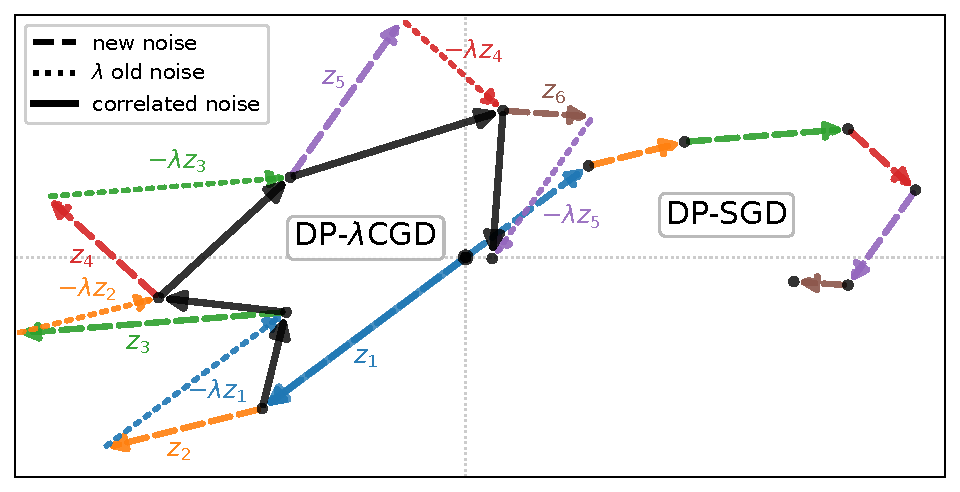
\includegraphics[width=1\linewidth]{images/subtraction_visualization.pdf}
    \caption{Visualization of noise correlation in \method. At each step, fresh noise $z_i$ is generated, and a $\lambda$-fraction of the previously added noise $z_{i-1}$ is canceled. In contrast, DP-SGD adds independent noise at each iteration. Although the per-iteration noise vectors in \method have larger variance, their correlation leads to partial noise cancellation, yielding a lower total variance. In this plot we set $\lambda=0.9$. The variance of the per-iteration noise is $1$ for DP-SGD and $\approx 1.67$ for \method, yet the variance of the cumulative noise in \method is about 44\% lower than in DP-SGD.}
    \label{fig:visualisation}
\end{figure}


In this paper, we propose \method, a matrix factorization and noise-correlation technique
that improves upon the utility of DP-SGD while remaining nearly as fast, requiring no
additional memory. Formally, we correlate the noise using a lower-triangular Toeplitz
strategy matrix $C_\lambda$ and its inverse (the corresponding correlation matrix)
$C_\lambda^{-1}$, defined entrywise as follows. For $i,j \in [n]$,
\begin{align}
\label{eq:C_lambda}
    &(C_\lambda)_{ij}
    \;:=\;
    \begin{cases}
        \lambda^{\,i-j}, & i \ge j,\\
        0, & i < j,
    \end{cases}\\
    &(C_\lambda^{-1})_{ij}
    \;:=\;
    \begin{cases}
        1, & i=j,\\
        -\lambda, & i=j+1,\\
        0, & \text{otherwise}.
    \end{cases}
\end{align}
Correlating the noise using $C_{\lambda}^{-1}$ is equivalent to subtracting a
$\lambda$-fraction of the noise added at the previous iteration (up to an overall
scaling determined by $\mathrm{sens}_{k,b}(C_{\lambda})$). We illustrate this noise
cancellation process in Figure~\ref{fig:visualisation}. Due to its simplicity, this correlation matrix has appeared as an exemplary factorization in several papers. It is referred to as ``Anti-PGD + damping'' in \citet{choquette2023correlated}, and it is used to illustrate noise correlation in the recent survey of \citet{pillutla2025correlated}. It also arises as a special case of the BandInvMF factorization in \citet{kalinin2025back}. \emph{However, it has not been studied beyond single-participation RMSE error, nor has it been used for practical DP training.}


To make our method memory-free, we observe that at each step we only need the noise
vector added in the previous iteration. As in essentially all practical private learning
pipelines, this noise is generated by a pseudo-random number generator (PRNG). Thus, by
storing the PRNG state from the previous iteration, we can roll back to that state,
regenerate the previous noise for cancellation, and then generate fresh noise exactly as
DP-SGD would. The drawback is that we must regenerate an additional noise vector each iteration, which
could introduce overhead. Empirically, however, this cost is negligible compared to the
rest of training (e.g., gradient computation): across multiple settings and model
families, \method runs within $1\%$ of the runtime of DP-SGD. See
Section~\ref{sec:noise_regeneration} for details.

Correlated noise can be combined with privacy amplification by subsampling. We use the
Balls-in-Bins subsampling scheme and its corresponding accountant \citep{choquette2024near}
to compute the resulting privacy guarantees. This allows improved utility at the same
target privacy level. For further discussion of the role of subsampling, see
Subsection~\ref{sub:amplification}.

Putting these ideas together, we outline the full procedure in
Algorithm~\ref{alg:method}. The algorithm takes $\lambda \in [0,1)$ as a hyperparameter; we discuss how to choose $\lambda$ in Section~\ref{sec:choice_of_lambda}.


\begin{algorithm}[t!]
\caption{\method}
\label{alg:method}
\begin{algorithmic}[1]
\REQUIRE Initialization $\theta_0 \in \mathbb{R}^d$, dataset $\mathcal{D}$, batch size $B$, clip norm $\zeta$, learning rate $\eta>0$, loss $\ell(\theta,d)$, parameter $\lambda \in [0,1)$, number of epochs $k$, target privacy level $\epsilon,\delta$, number of iterations $n$, pseudorandom noise generator $\mathrm{gen}$.
\STATE Construct matrix $C_{\lambda} = \mathrm{LTT}(1, \lambda, \dots, \lambda^{n-1})$
\IF{use Balls in Bins accountant}
    \STATE Compute noise multiplier $\sigma = \mathrm{BnB}(C_{\lambda}, k, \epsilon, \delta)$
    \STATE Randomly allocate batches $D_1, \dots, D_{|\mathcal{D}|/B}$ 
\ELSIF{no amplification}
    \STATE $\sigma = \mathrm{sens}_{k,b}(C_{\lambda})\,\sigma_{\epsilon,\delta}$, where $\sigma_{\epsilon,\delta}$ is from the Gaussian mechanism
\ENDIF
\STATE $\mathrm{GSt}_1 \gets \mathrm{gen.get\_state()}$
\STATE $Z_0 \xleftarrow{} 0$
\FOR{$i=1$ to $n$}
    \STATE \qquad \COMMENT{Sample batch}
    \IF{use Balls in Bins subsampling}
        \STATE $S_i = D_{i \bmod (n/k)}$
    \ELSIF{no amplification}
        \STATE $S_i = \{d_{(i-1)B \bmod |\mathcal{D}|},\dots,d_{(iB-1) \bmod |\mathcal{D}|}\}$
    \ENDIF
    \FOR{$j=1$ to  $|S_i|$}
        \STATE $g_j \gets \nabla_\theta \ell(\theta_{i-1}, d_j)$
        \STATE $\tilde g_j \gets \min\!\bigl(1, \frac{\zeta}{\|g_j\|}\bigr)\, g_j$ \quad \COMMENT{per-example clipping}
    \ENDFOR
    \STATE $x_i \gets \sum_{j=1}^{|S_i|} \tilde g_j$ \qquad \COMMENT{aggregate clipped gradients}
    \IF{$i \ne 1$}
    \STATE $\mathrm{gen} \gets \mathrm{gen.set\_state(\mathrm{GSt}_{i -1} )}$
    \STATE $Z_{i-1} \sim \mathrm{gen}()$ \qquad \COMMENT{regenerate noise}
    \ENDIF
    \STATE $\hat x_i \gets x_i - \zeta\sigma \lambda Z_{i-1}$
    \STATE $\mathrm{GSt}_i \gets \mathrm{gen.get\_state()}$
    \STATE $Z_i \sim \mathrm{gen}()$ \qquad \COMMENT{generate fresh noise}
    \STATE $\hat x_i \gets \hat x_i + \zeta\sigma Z_i$
    \STATE $\theta_i \gets \theta_{i-1} - \frac{\eta}{B}\hat x_i$ \qquad \COMMENT{model update}
\ENDFOR
\STATE \textbf{return} $\theta_n$
\end{algorithmic}
\end{algorithm}


We establish several properties of the \method with respect to the RMSE and MaxSE error
metrics. We begin by analyzing the MaxSE error, which is characterized in the following
lemma.

\begin{restatable}{lemma}{MaxSEBound}
\label{lem:MaxSEBound}
The MaxSE of \method, optimized over $\lambda \in [0,1)$, satisfies
\begin{equation}
    \!\!\inf_{\lambda \in [0,1)}\!\!
    \|A C_{\lambda}^{-1}\|_{2 \to \infty}
    \cdot \mathrm{sens}_{k,b}(C_{\lambda})
    = O\!\big(k + \sqrt{k}\, n^{1/4}\big) 
\end{equation}
\end{restatable}

Since RMSE is upper bounded by MaxSE for any factorization, the same bound also applies to
the RMSE of \method. 

The $O(n^{1/4})$ term for the single-participation setting, as well as the optimal factorization error $O(k+\sqrt{k}\log n)$, were derived in \citet{kalinin2025back}. Here, we extend the factorization result to the multi-participation regime. Our bound improves over the trivial (i.e., DP-SGD) factorization, which yields error $O(\sqrt{nk})$, though it remains weaker than the optimal factorization error.


Despite this, we will show that improved RMSE does not always translate into better model
performance. In particular, in certain regimes, \method outperforms factorizations with
smaller RMSE.

The \method is the first framework that allows us to establish structural properties of
optimal factorizations. In particular, we show that the minimizer of the MaxSE objective is
always larger than the minimizer of the RMSE objective, which makes RMSE a more practically
relevant metric. We discuss this phenomenon in detail in
Section~\ref{sec:choice_of_lambda}.


\begin{restatable}{lemma}{MaxSEvsRMSEMinimizerInequality}
\label{lem:method_minimizer_inequality}
For \method, a minimizer of MaxSE is always at least as large as a minimizer of RMSE.
\end{restatable}


\section{Noise Regeneration}
\label{sec:noise_regeneration}

\begin{figure}[t]
    \centering
    \begin{subfigure}[t]{\linewidth}
        \centering
        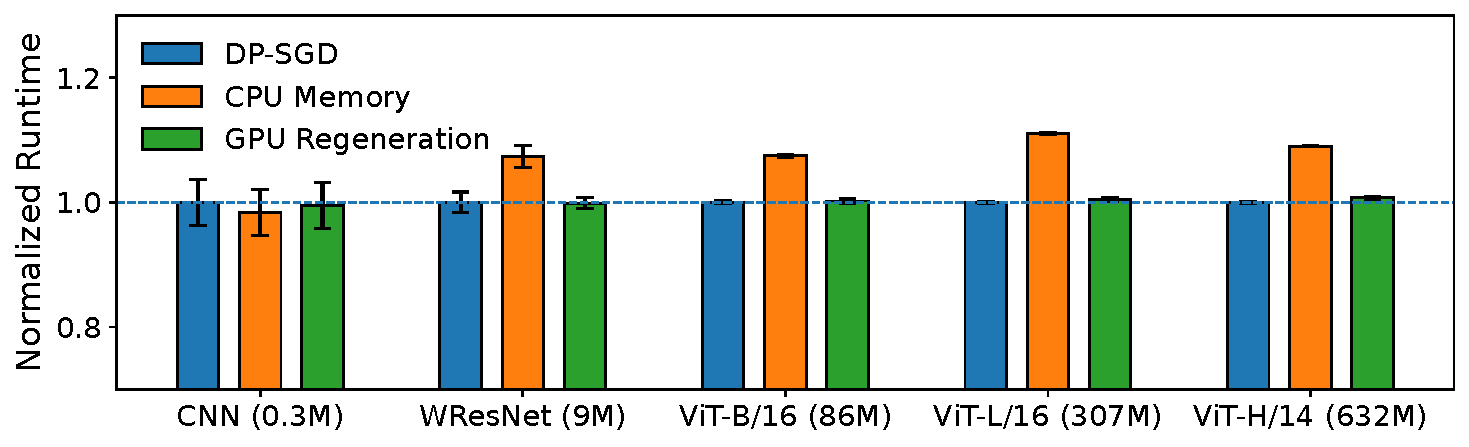
\includegraphics[width=1\linewidth]{images/normalized_runtime_bw2.pdf}
        \caption{CIFAR-10 runtime for one epoch.}
        \label{fig:time_comparison_cifar}
    \end{subfigure}

    \vspace{0.75em}

    \begin{subfigure}[t]{\linewidth}
        \centering
        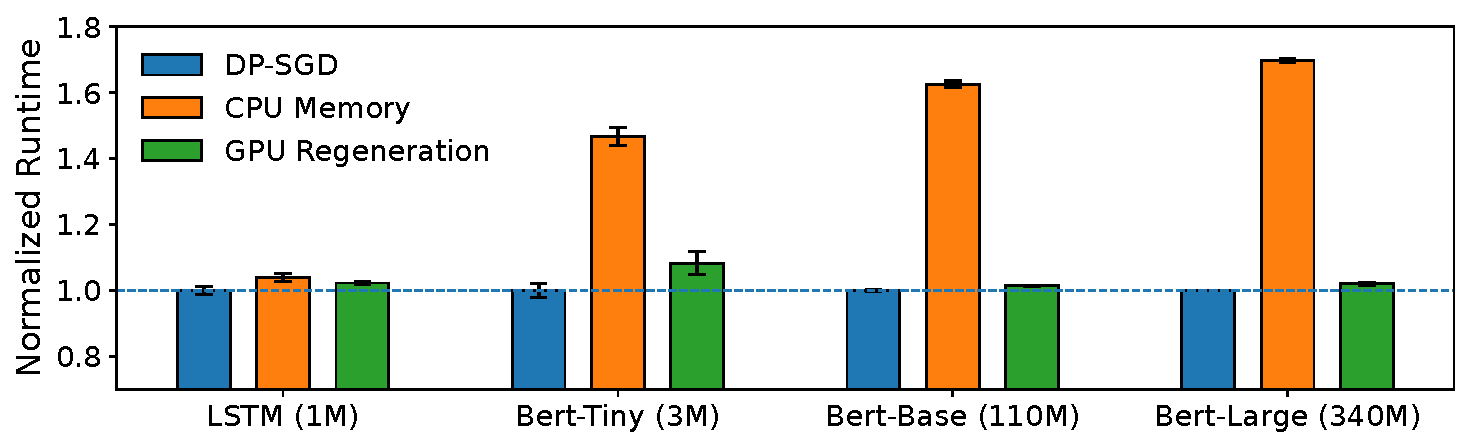
\includegraphics[width=1\linewidth]{images/normalized_runtime_IMDB.pdf}
        \caption{IMDB fine-tuning runtime for one epoch.}
        \label{fig:time_comparison_imdb}
    \end{subfigure}

    \caption{Runtime for one epoch, comparing DP-SGD runtime using the Opacus implementation versus storing the noise on the CPU and regenerating it on the GPU using pseudorandomness.}
    \label{fig:time_comparison}
\end{figure}

Modern private machine learning uses pseudo-random number generators (PRNGs) to generate noise.
A PRNG has a small \emph{state} that determines its next output as well as its next state.
The state is typically initialized to a random ``seed'' value using hardware-supported random number generation, and the whole sequence of random values is determined by the initial state.
So-called \emph{counter-based} PRNGs have a fixed state given by a seed $s$ and take a counter $i$ as input to generate the $i$th random value (that is, it implements a hash function from counters to random values).
PyTorch uses the counter-based {\tt Philox4x32-10} pseudorandom number generator~\cite{salmon2011parallel} on CUDA devices, which deterministically maps a 64-bit seed and a 128-bit counter to random values, enabling reproducible and scalable parallel random number generation on GPUs.


\paragraph{Regeneration.}
Previous approaches to noise correlation described in the literature required storing noise vectors generated in earlier steps, which can require substantial memory that may not be available on the GPU. 
Alternatively, one can store the noise on the CPU and transfer it to the GPU, but this incurs substantial overhead.
By storing a state of the PRNG it is possible to go back and ``replay'' any part of the pseudorandom sequence, trading the space for the time needed to regenerate randomness.
Although such noise regeneration is not discussed in the literature to our best knowledge, the reference code of \citet{choquette2022multi} implements such ``on the fly'' noise.\footnote{\url{https://github.com/google-research/federated/blob/master/dp_matrix_factorization/matrix_factorization_query.py\#L190}} 
However, their implementation reconstructs the entire noise sequence from the first iteration each time, which is computationally expensive.

Our proposed \method, as well as Banded Inverse Matrix Factorization and Banded Inverse Square Root with small bandwidth \citep{kalinin2025back}, needs to access only a small number of the most recent noise vectors. 
This makes it efficient to regenerate noise on the fly without storing the history. Note that banded methods such as Banded Matrix Factorization \citep{scalingmckenna2024} and Buffered Linear Toeplitz \citep{dvijotham2024efficient, hasslefree2024} can correlate noise using a relatively small in-memory buffer; however, at each step the correlated noise depends on components originating from the very first iteration. Regenerating the full sequence at every step would be impractical (see Table~\ref{tab:noise_time_buffer} for the time and space requirements).


\paragraph{Discussion.}
The random values generated by Philox and other popular high-performance PRNGs used in machine learning frameworks pass statistical tests of randomness but are not cryptographically secure. This potentially weakens the privacy protection, but since the de-facto standard is to not use slower, cryptographically secure PRNGs~\cite{egan2024highspeed} we will follow this standard.
Using slower PRNGs may shift the trade-off between the cost of storing noise values and regenerating them.

\paragraph{Evaluation.}
We evaluate GPU-based noise regeneration against DP-SGD, as well as against an alternative that stores and correlates noise on the CPU. In Fig.~\ref{fig:time_comparison}, we report the relative time per epoch on CIFAR-10 with batch size $512$ for model sizes ranging from a small CNN with $0.3$M parameters to ViT-H/14 with $632$M parameters \citep{dosovitskiy2021vit}. We also evaluate on the IMDB sentiment analysis task using an LSTM and a family of BERT models \citep{devlin2019bert}, with a smaller batch size of $128$. Our results indicate almost no overhead when running \method compared to DP-SGD (less than $1\%$ on CIFAR-10 and $2\%$ on IMDB). By contrast, when noise is stored on the CPU and transferred to the GPU, the overhead increases to nearly $10\%$ in the CIFAR-10 experiments and $70\%$ on IMDB.


\begin{figure*}[t]
    \centering
    
    \begin{subfigure}{0.30\linewidth}
        \centering
        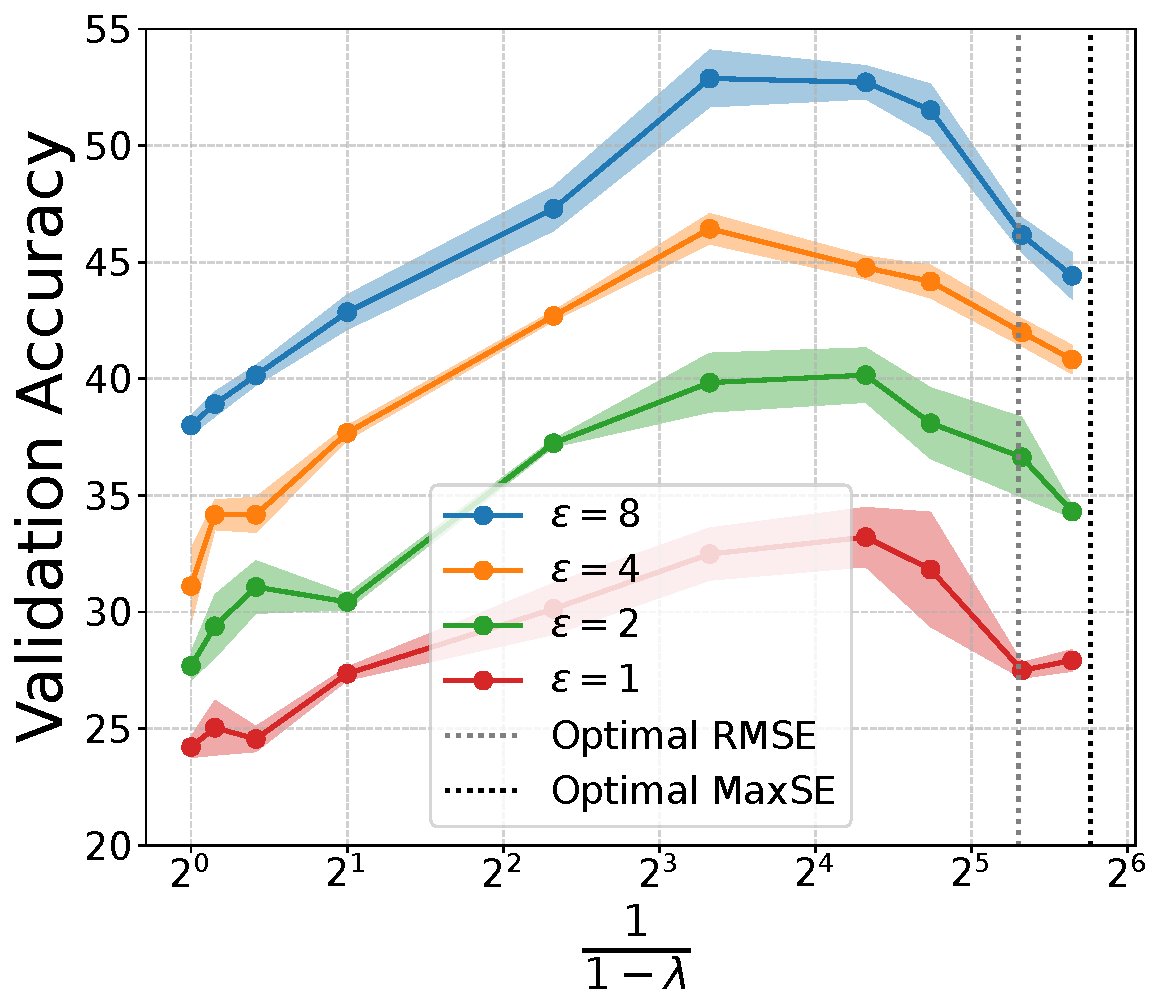
\includegraphics[width=\linewidth]{images/cifar10_bandwidth_2_B_128_k_10.pdf}
        \caption{CIFAR-10: $B= 128$, $k =10$}
    \end{subfigure}
    \begin{subfigure}{0.30\linewidth}
        \centering
        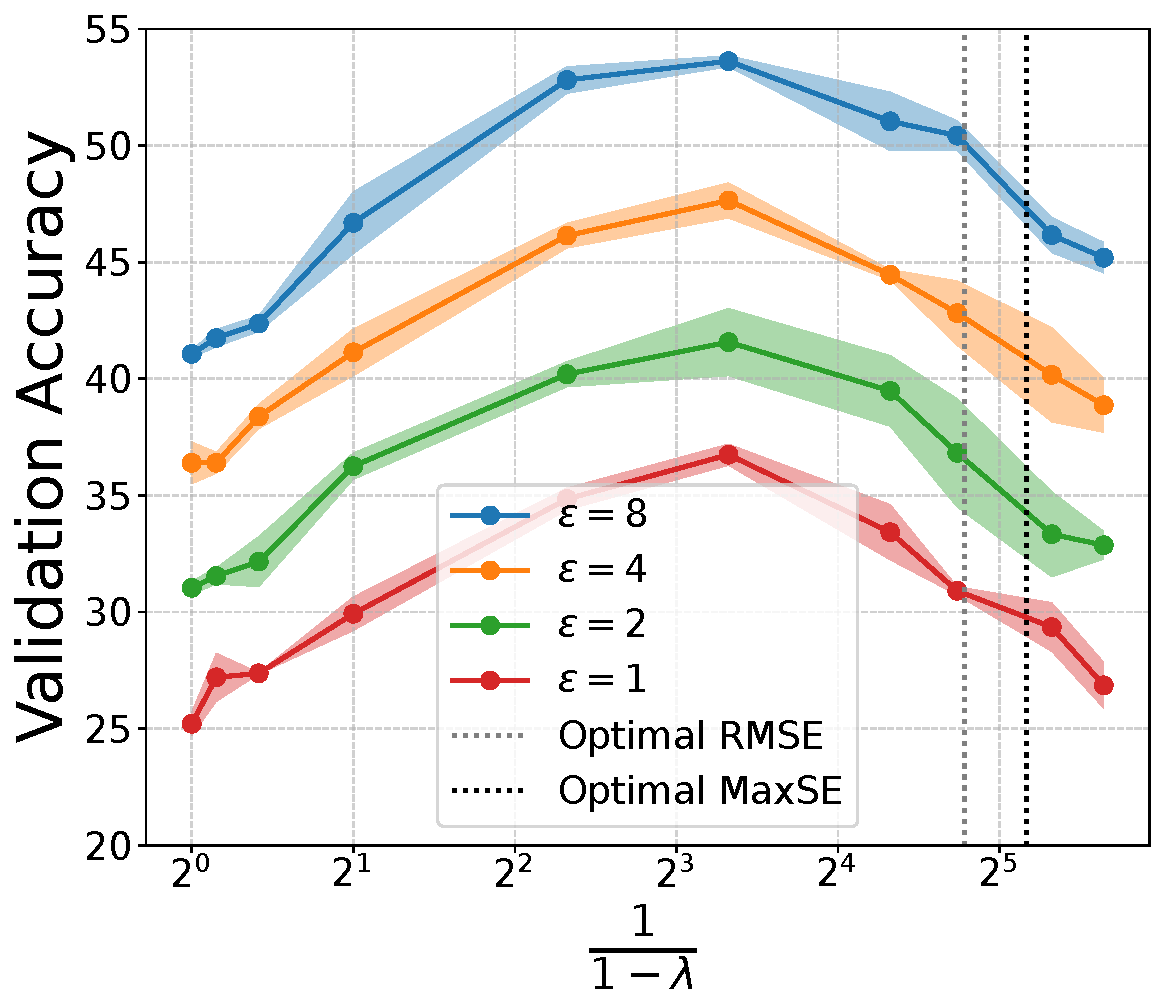
\includegraphics[width=\linewidth]{images/cifar10_bandwidth_2_B_256_k_10.pdf}
        \caption{CIFAR-10: $B=256$, $k=10$}
    \end{subfigure}
    \begin{subfigure}{0.30\linewidth}
        \centering
        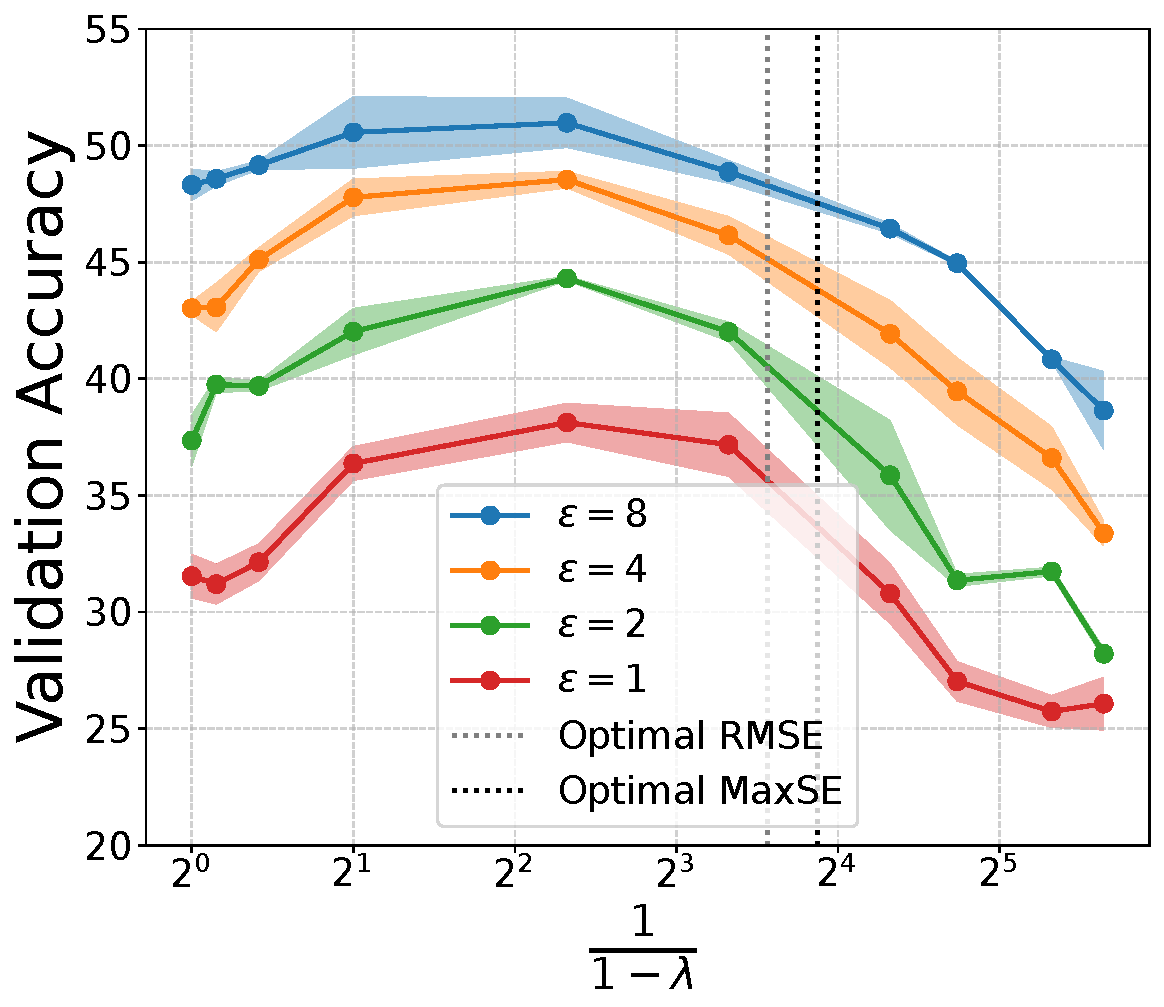
\includegraphics[width=\linewidth]{images/cifar10_bandwidth_2_B_1024_k_10.pdf}
        \caption{CIFAR-10: $B=1024$, $k=10$}
    \end{subfigure}

    \begin{subfigure}{0.30\linewidth}
        \centering
        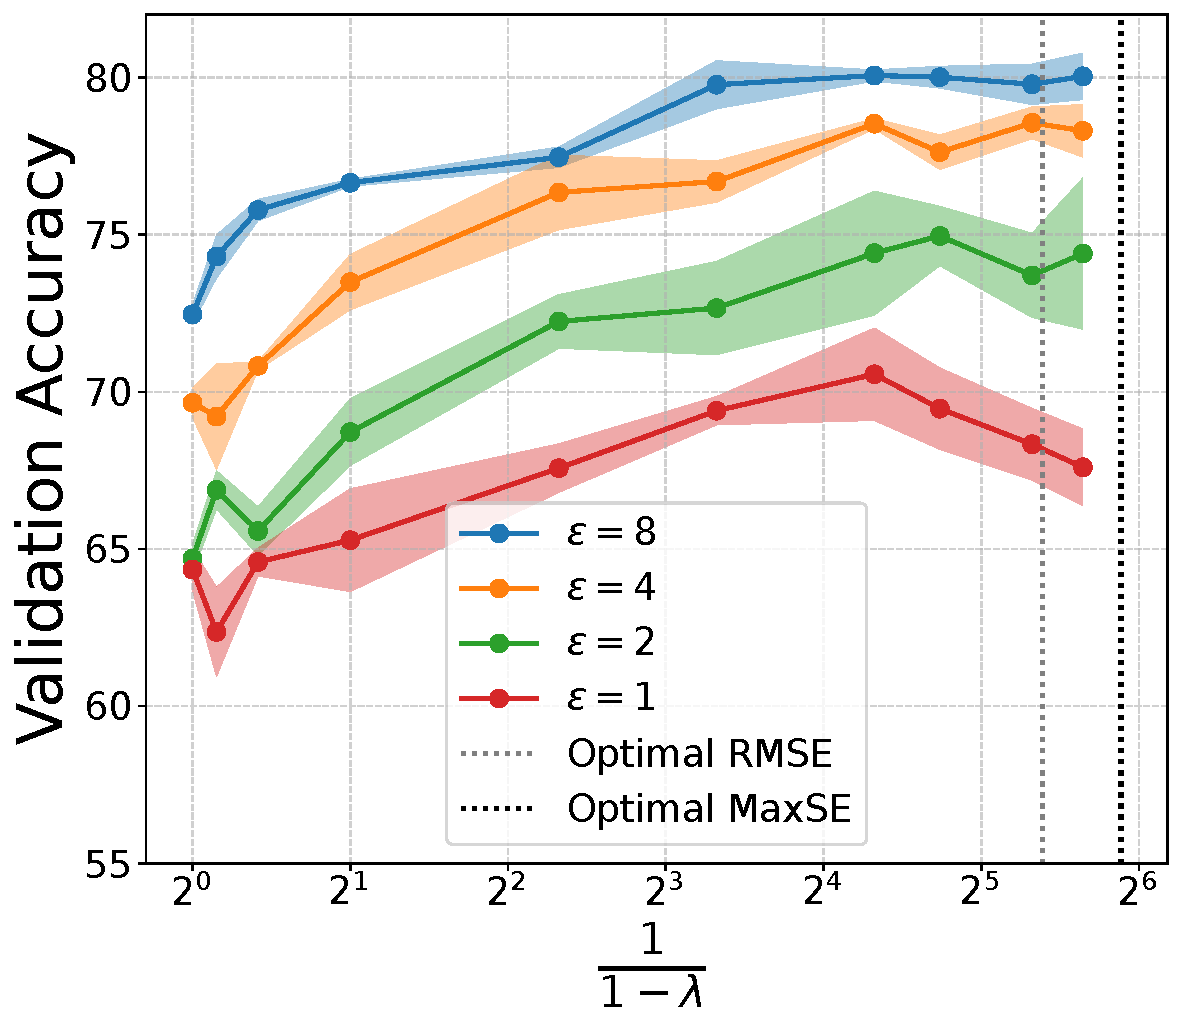
\includegraphics[width=\linewidth]{images/imdb_bandwidth_2_B_64_k_10.pdf}
        \caption{IMDB: $B=64$, $k=10$}
    \end{subfigure}
    \begin{subfigure}{0.30\linewidth}
        \centering
        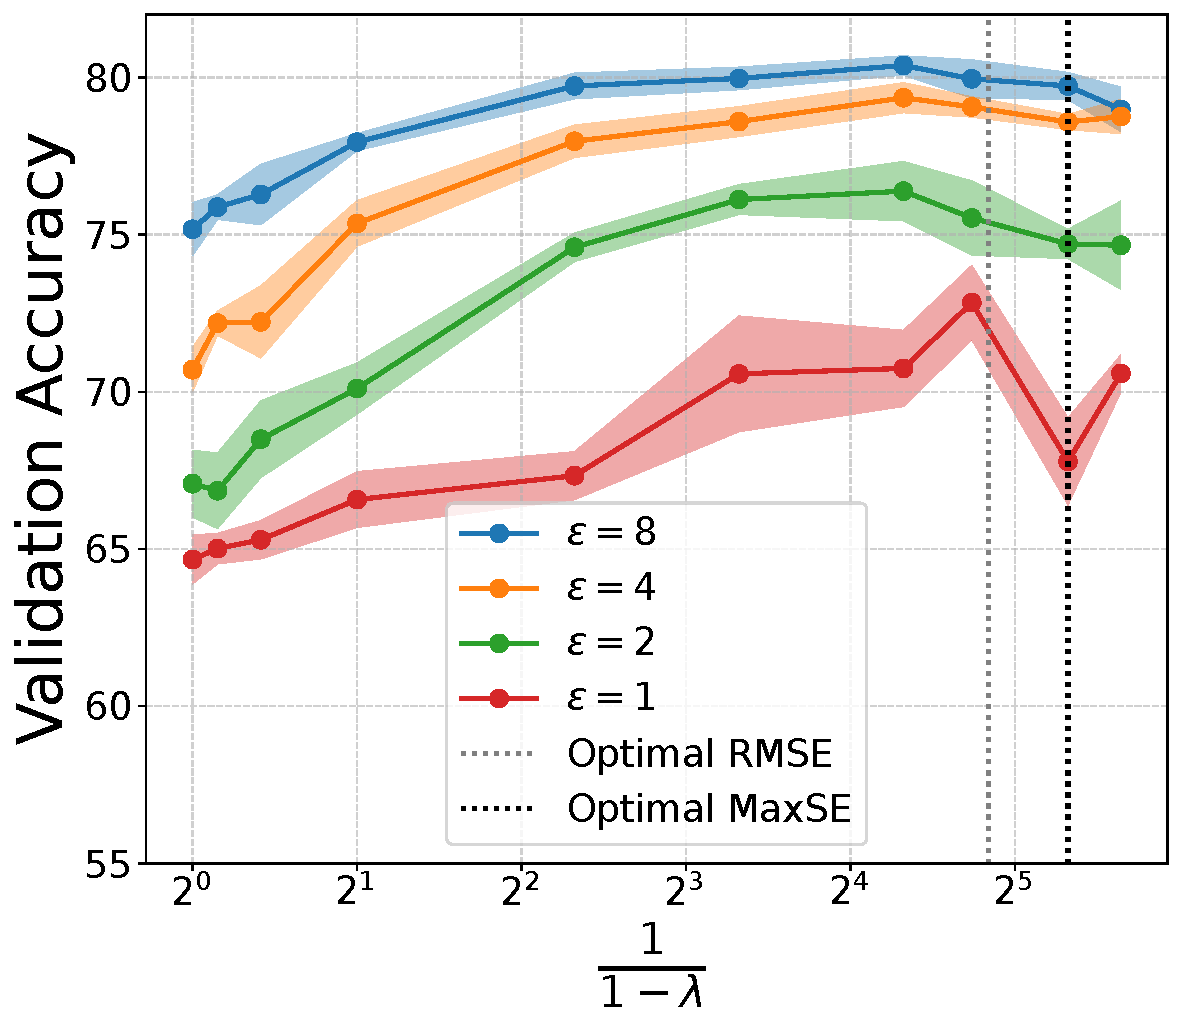
\includegraphics[width=\linewidth]{images/imdb_bandwidth_2_B_128_k_10.pdf}
        \caption{IMDB: $B=128$, $k=10$}
    \end{subfigure}
    \begin{subfigure}{0.30\linewidth}
        \centering
        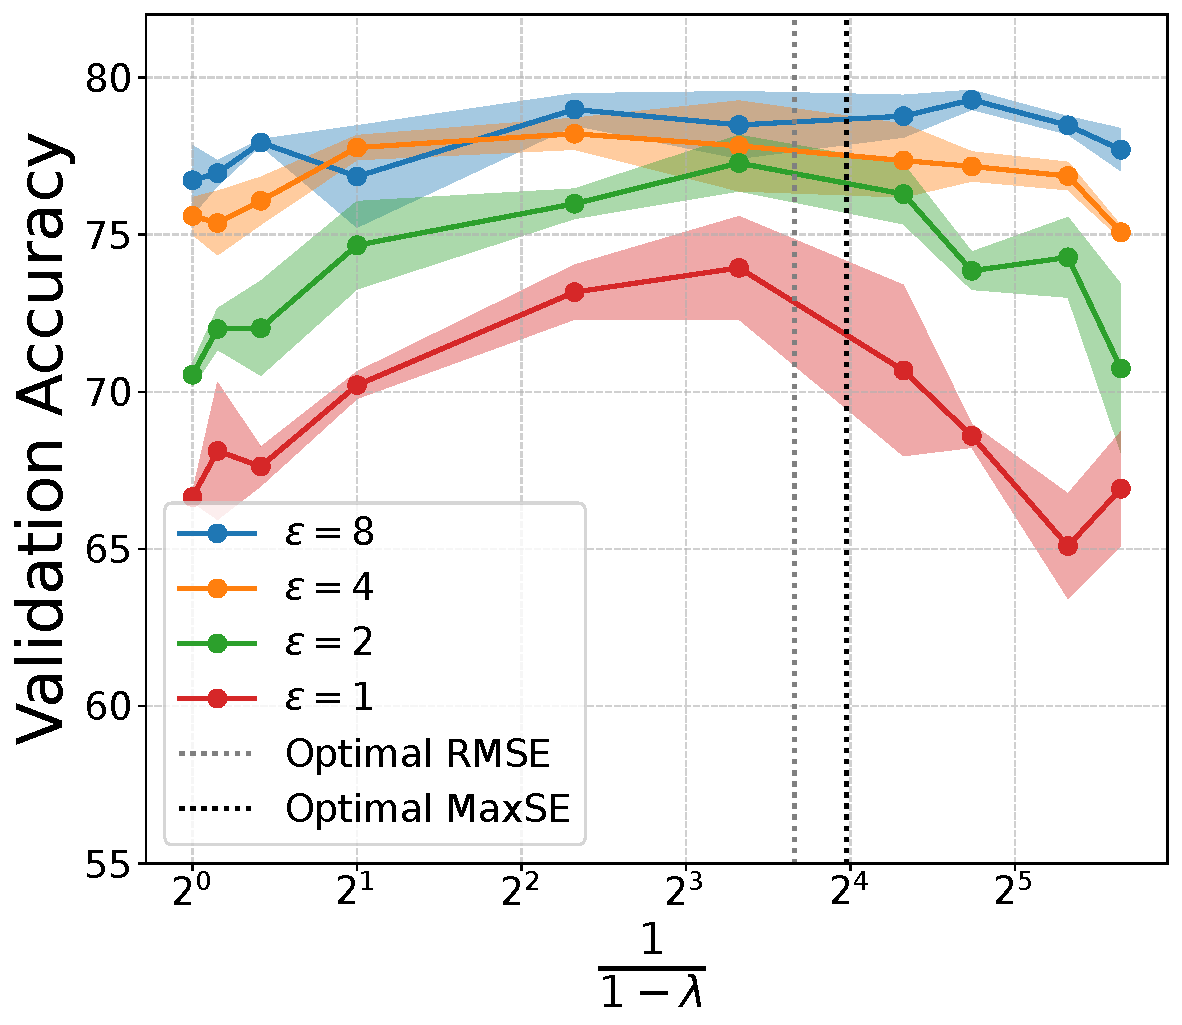
\includegraphics[width=\linewidth]{images/imdb_bandwidth_2_B_512_k_10.pdf}
        \caption{IMDB: $B=512$, $k=10$}
    \end{subfigure}    
    

    \caption{ Validation accuracy for different values of the parameter $\lambda$ in \method.
The first row shows a CNN model trained on CIFAR-10 for $k=10$ epochs, using different batch sizes $B$.
The second row shows fine-tuning of the BERT-tiny model on the IMDB sentiment analysis dataset.
For each point, we tune the learning rate; error bars are computed based on three runs.
The lower and upper plots correspond to almost the same training configuration in terms of $n$, $k$, $B$, and the correlation matrix used, but demonstrate different qualitative behavior. }
    \label{fig:choice_of_lambda}
\end{figure*}


In Tables~\ref{tab:runtime_comparison} and~\ref{tab:runtime_comparison_imdb} in the appendix, we report the absolute runtime for different bandwidths, where bandwidth $2$ corresponds to \method and larger bandwidths correspond to Banded Inverse Matrix Factorization \citep{kalinin2025back}. 
%
The tables show that regenerating a small noise buffer ($p=4$ or $p=16$) increased the cost by at most $8\%$, whereas CPU storage increased runtime by about $147\%$.



\section{How to choose the value $\lambda$?}
\label{sec:choice_of_lambda}

The best value of $\lambda$ for \method can depend on the batch size, the number of
epochs, the target privacy level, whether amplification by subsampling is used, and,
ultimately, the learning problem (\eg, the loss function and data distribution). 
%
To study how to choose this parameter in practice, we report results of an extensive sweep over $\lambda$ in Figure~\ref{fig:choice_of_lambda}.

Figure~\ref{fig:choice_of_lambda} reports results \emph{without} amplification, which
allows us to characterize the behavior of RMSE- and MaxSE-optimal factorizations
theoretically; for the role of subsampling, see Subsection~\ref{sub:amplification}.
We make three empirical observations. First, the best choice of $\lambda$ appears to be
task-dependent: under similar training settings and identical matrices, the optimal
$\lambda$ differs substantially between training a CNN on CIFAR-10 and fine-tuning
BERT-tiny on IMDB. In particular, for CIFAR-10 the optimal $\lambda$ is much smaller
than the value suggested by the RMSE-optimal factorization. Moreover, as shown in
By Lemma~\ref{lem:method_minimizer_inequality}, the minimum value of the MaxSE objective is always larger than the minimum value of the RMSE objective. Consequently, MaxSE is farther from the optimum and is therefore a less suitable objective for \method. Second, the
optimal $\lambda$ is relatively insensitive to the privacy level across the range we
tested. Third, as the batch size increases, the RMSE-optimal factorization approaches
DP-SGD. However, Figure~\ref{fig:experiments_fixed_batch_size} in the appendix shows that, for a fixed non-full batch size, increasing the number of epochs pushes the optimal mechanisms further away from DP-SGD (e.g. the optimal $\lambda$ increases). This suggests that even in long training runs, common in high-performance DP-SGD training, the benefit of matrix factorization, and \method in particular, continues to grow.

In the rest of this subsection, we prove several theoretical results on optimal factorizations in the full-batch regime. In the limit, DP-SGD is an optimal factorization in a variety of settings, which suggests that, for a fixed number of epochs, larger batch sizes lead to smaller optimal values of $\lambda$.



To theoretically understand the dependence on the batch size, we develop a theory for the
multi-participation error in the full-batch setting, corresponding to $b = 1$ and $k = n$.
The optimal factorization results of \citet{kalinin2025back} imply that, asymptotically,
DP-SGD (i.e., the trivial factorization) is optimal in this regime, with RMSE scaling as
$O(n)$. Here, we go beyond asymptotic analysis and study constant-optimal factorizations.

We first show that DP-SGD is \textbf{not} constant-optimal under the RMSE metric. In
particular, there exists the optimal diagonal factorization with weights $(n - j + 1)^{1/4}$ that
achieves a smaller error constant among diagonal factorizations. This improvement is obtained by injecting larger noise
into later estimates, which may be undesirable in practice (see Remark 4.10 from \citet{pillutla2025correlated}) since model training typically
prioritizes higher accuracy for the final model. Both the trivial and weighted diagonal
factorizations are within $21\%$ of the lower bound that we establish, with the weighted
diagonal factorization improving upon DP-SGD by approximately $6\%$. See the following
theorem for the formal statement.

\begin{theorem}[Constant-optimal bounds for multi-participation error, full-batch regime]
\label{thm:full_batch_constants}
Let $b = 1$ and $k = n$, and let $A \in \mathbb{R}^{n \times n}$ be the prefix-sum matrix.

The trivial factorization $C = I$ yields
\begin{equation}
    \mathrm{RMSE}(A, I)
    \;=\;
    \sqrt{\frac{n(n+1)}{2}}
    \;\sim\;
    \frac{n}{\sqrt{2}}.
\end{equation}
This error is approximately $6\%$ larger than that of the optimal diagonal factorization
$C_{\mathrm{diag}} = \mathrm{diag}\!\big( (n - j + 1)^{1/4} \big)_{j=1}^n$, for which
\begin{equation}
    \mathrm{RMSE}(A C^{-1}_{\mathrm{diag}}, C_{\mathrm{diag}})
    \;=\;
    \frac{1}{\sqrt{n}} \sum_{j=1}^n \sqrt{j}
    \;\sim\;
    \frac{2n}{3}.
\end{equation}

Moreover, for any factorization $A = BC$, the following lower bound holds:
\begin{equation}
    \mathrm{RMSE}(B, C)
    \;\ge\;
    \sqrt{\frac{(n+1)(2n+1)}{6}}
    \;\sim\;
    \frac{n}{\sqrt{3}}.
\end{equation}
\end{theorem}

We conjecture that the diagonal factorization is constant optimal\footnote{Note that in Proposition 4.9 from \citet{pillutla2025correlated} the diagonal factorization is stated to be constant optimal, however they consider $b$-banded class of factorizations, which consists only of diagonal matrices in the full-batch regime. We do not have such restrictions.}; however, there
remains an approximately $15\%$ gap to the lower bound. This establishes that DP-SGD is not
numerically optimal under the RMSE metric. Nevertheless, DP-SGD could be optimal under the
MaxSE metric. 

\begin{lemma}(Proposition 3.11 from \citet{pillutla2025correlated})
\label{lem:dp_sgd_maxse_optimality}
The trivial factorization $B = A$, $C = I$ is optimal among all
factorizations for $b = 1$ and $k = n$ in dimension $d = 1$.
\end{lemma}

Combining the Lemma~\ref{lem:dp_sgd_maxse_optimality} with  Proposition E.1 in \citet{choquette2023amplified} it follows that DP-SGD is optimal in any dimension $d\ge 1$ among factorizations with positive elements in the strategy matrix $C$, resulting in the following corollary.

\begin{corollary}
The trivial factorization $B = A$, $C = I$ is optimal for \method under the RMSE
and MaxSE metrics for $b = 1$ and $k = n$.
\end{corollary}
\begin{proof}
From Lemma~\ref{lem:dp_sgd_maxse_optimality}, it follows that the trivial
factorization is optimal for \method in MaxSE metric since for any $\lambda > 0$ the values in $C_{\lambda}$ \eqref{eq:C_lambda} are positive.
From Lemma~\ref{lem:method_minimizer_inequality}, it follows that the optimal value of
$\lambda$ for the RMSE metric is bounded by that for the MaxSE metric, which is
$0$ in this case. Therefore, $\lambda = 0$, i.e., the trivial factorization is
also optimal for RMSE.
\end{proof}



\begin{figure*}[t]
    \centering
    \begin{minipage}{0.65\textwidth}
    %\begin{subfigure}[t]{0.48\linewidth}
        \begin{minipage}{.47\textwidth}
        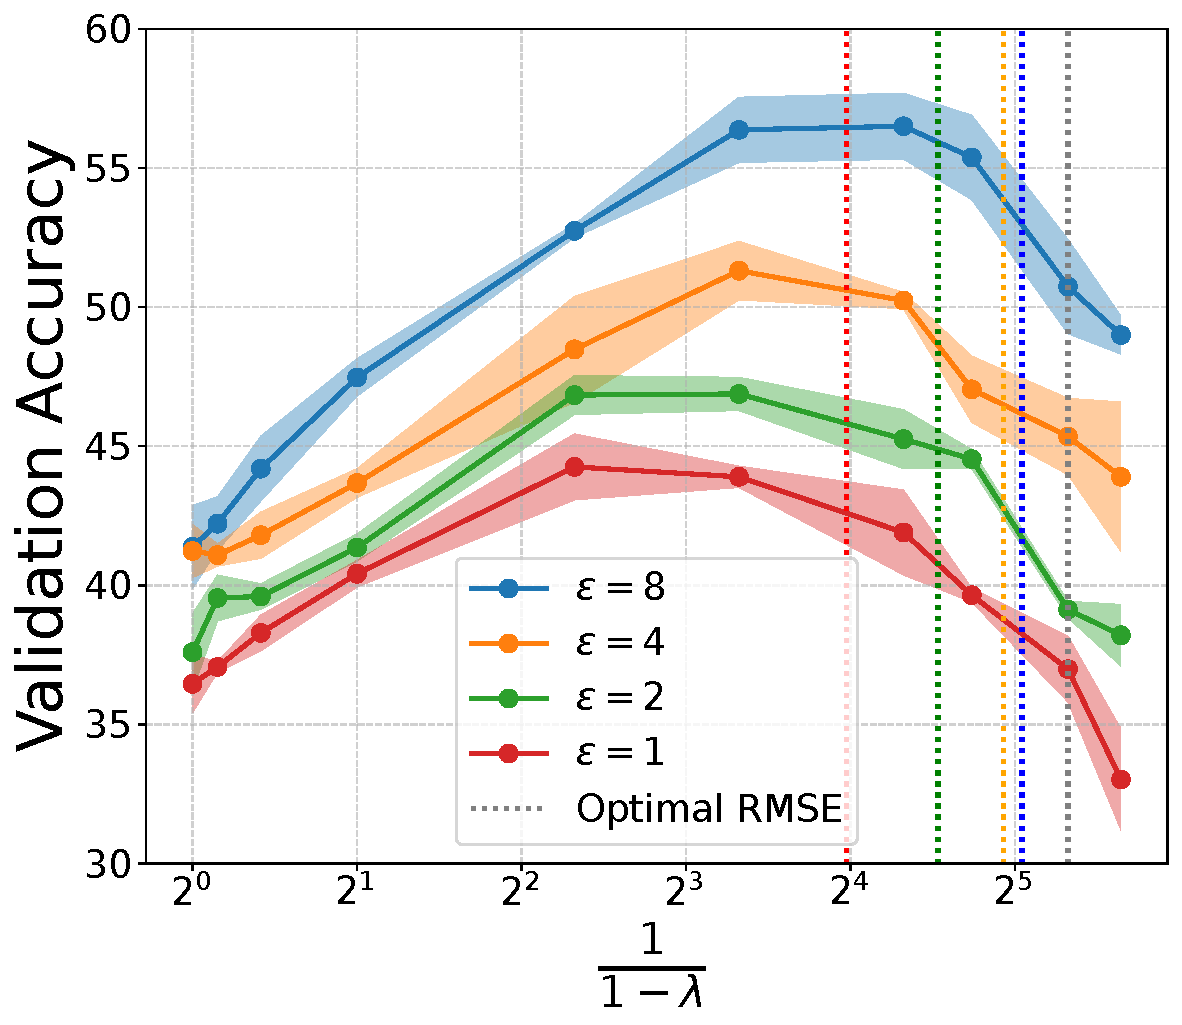
\includegraphics[height=.8\linewidth]{images/cifar10_bandwidth_2_B_128_k_10_amplified.pdf}
        
        \centerline{\footnotesize CNN on CIFAR-10 $B=128$, $k=10$.}
        \end{minipage}
        \quad
        \begin{minipage}{.47\textwidth}
        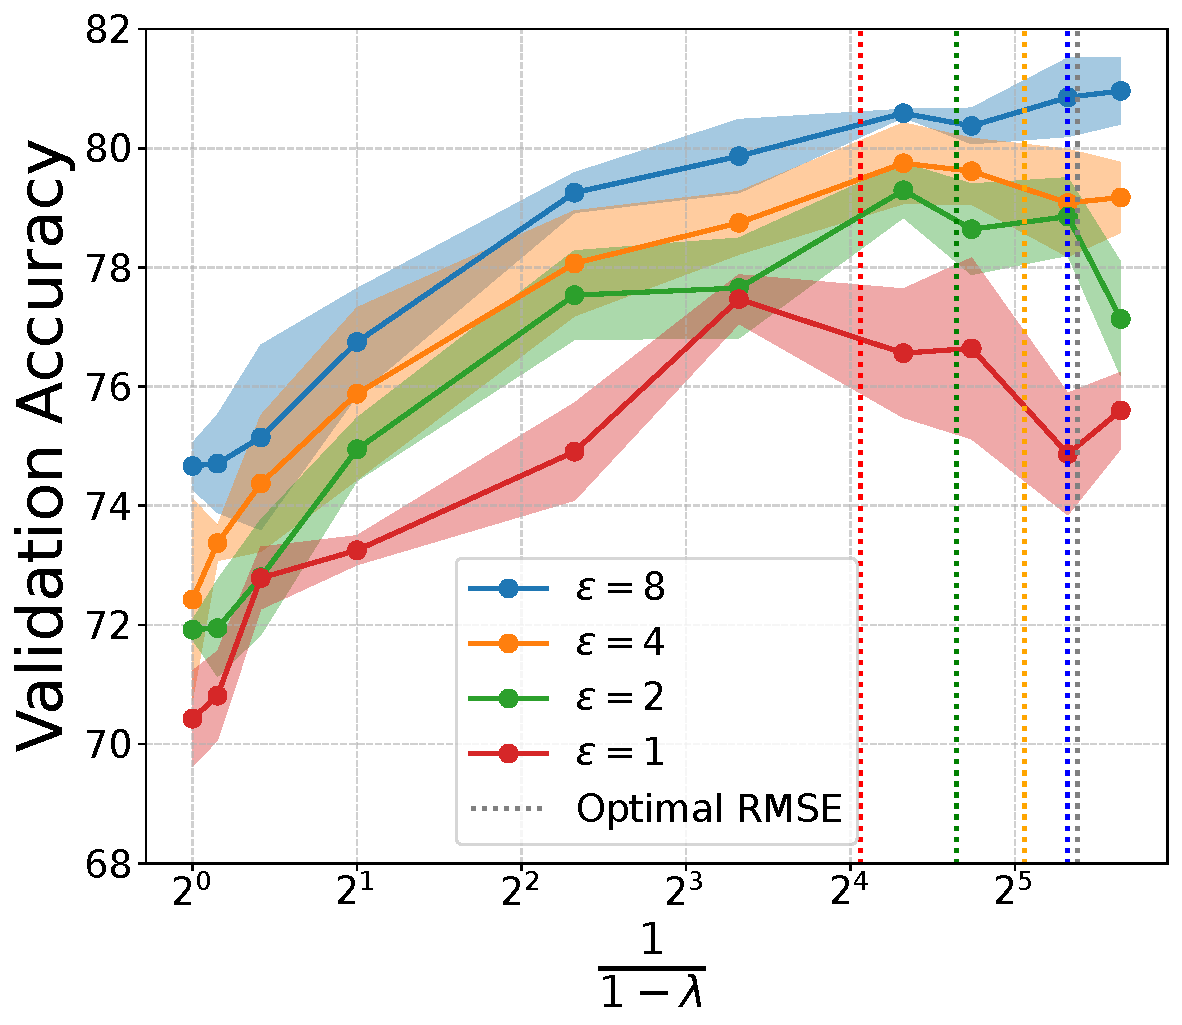
\includegraphics[height=.8\linewidth]{images/IMDB_bandwidth_2_B_64_k_10_amplified.pdf}
        
        \centerline{\footnotesize BERT-Tiny on IMDB $B=64$, $k=10$.}
        \end{minipage}
        %\label{fig:imdb_with_amplification}
    \caption{Validation accuracy of \method with Balls-in-Bins amplification by subsampling for different values of $\lambda$. Vertical lines indicate the optimal values based on the amplified RMSE, suggesting that Balls-in-Bins prefers smaller values of $\lambda$. However, the value of $\lambda$ that is optimal for accuracy is even lower, at least for CIFAR-10 training.}
    \label{fig:amplification_results}
    \end{minipage}
    \quad
    \begin{minipage}{0.31\textwidth}
    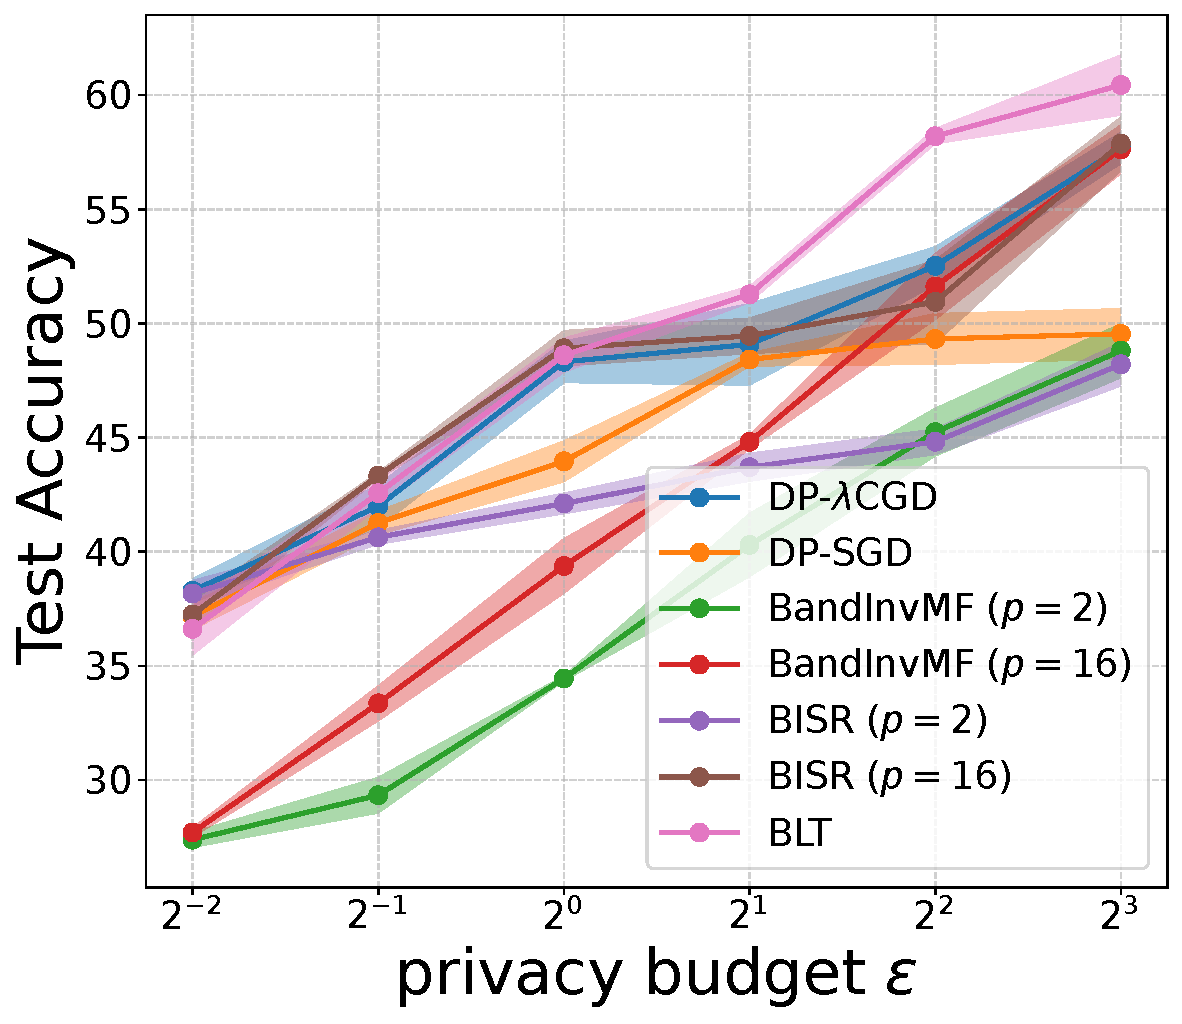
\includegraphics[height=.8\linewidth]{images/accuracy_vs_epsilon_all_methods.pdf}
    \caption{Test accuracy on CIFAR- ($B=128$, $k=10$; error bars based on three runs). We compare DP-SGD with Poisson subsampling, \method, BISR, BandInvMF, and BLT with Balls-in-Bins subsampling. See main body for details. 
}
    \label{fig:method_comparison_cifar_10}
    \end{minipage}
\end{figure*}


\subsection{Amplification}
\label{sub:amplification}


The most common amplification scheme for DP-SGD is Poisson subsampling \citep{Abadi, koskela2020computing, zhu2022optimal}, in which each batch is formed independently and each element is included with a probability determined by the expected batch size. This method provides the strongest known privacy guarantees among sampling schemes. However, it has notable limitations. In expectation, nearly one third of the data (specifically, a fraction $1/e$) does not participate in each epoch. Moreover, Poisson subsampling is difficult to implement efficiently at scale, since forming each batch would require scanning the entire dataset and independently deciding whether to include each element. This leads to the common but undesirable practice of training with shuffling while reporting privacy guarantees under Poisson subsampling \citep{lebeda2025avoiding, beltran2024towards}.

To address these issues, an alternative sampling scheme was proposed, known as Balls in Bins (BnB) \citep{chua2024balls, choquette2024near} or random allocation \citep{feldman2025privacy}. In this approach, one first specifies the number of batches in an epoch and then assigns each data point to a random batch. This guarantees that every sample participates once per epoch, and by preprocessing the dataset, one can efficiently construct batches for multi epoch training. 

Balls-in-Bins amplification by subsampling can also be applied to matrix factorization \citep{choquette2024near} for any correlation matrix. We use it for \method, as it is also the only currently available amplification scheme that is applicable to banded inverse matrices. Poisson subsampling can be applied to $b$-min-separated participation for the banded matrix case \citep{choquette2023amplified}, and it can also be applied to general matrices, although the existing analysis does not scale to the matrix sizes used in our experiments \citep{choquette2023privacy}. The development of improved amplification techniques that are suitable for banded inverse matrices is an important direction for future research. Since our method is orthogonal to the choice of amplification scheme, any such analysis can be incorporated seamlessly into our mechanism.
 

\citet{choquette2024near} compute the privacy level using Monte Carlo sampling. This procedure is effective in practice but acts as a black box and does not allow us to argue theoretically about its properties. We therefore study the effect of amplification numerically. Our experiments show that amplification by Balls in Bins subsampling prefers smaller values of $\lambda$ than those that would be chosen based solely on RMSE. In particular, the values that minimize the amplification-aware RMSE: $\tfrac{1}{\sqrt{n}}\|B\|_F \cdot \sigma$ are closer to the optimal factorization for \method\ than those obtained using RMSE alone. See Figure~\ref{fig:amplification_results} for an illustration.



\section{Experiments}
We compare \method, amplified via Balls-in-Bins subsampling, to other memory-efficient alternatives, including DP-SGD with Poisson subsampling (a commonly used amplification that empirically yields a slightly lower noise multiplier) and the banded inverse factorizations Banded Inverse Matrix Factorization (BandInvMF) and Banded Inverse Square Root (BISR) \citep{kalinin2025back} with bandwidths $2,4,16$.
 We also include Buffered Linear Toeplitz (BLT)  factorization \citep{dvijotham2024efficient}; although BLT cannot be run efficiently without additional memory, we find it to be a competitive low-memory approach, requiring to store a small buffer of $4-5$ vectors. In Table~\ref{tab:eps_all}, we compare the methods using the RMSE metric, with and without amplification. In the table, we also report banded factorizations such as Banded Matrix Factorization (BandMF) \citep{scalingmckenna2024} and Banded Square Root (BSR) \citep{kalinin2024}; however, they do not perform competitively at small bandwidths ($2$, $4$, or even $16$).

Figure~\ref{fig:method_comparison_cifar_10}
reports the results of CNN training on the 
CIFAR-10 dataset (for hyperparameters, see Table~\ref{tab:hyperparams} in the appendix).
%
Our proposed \method outperforms DP-SGD even in the high-privacy regime $\epsilon=1/4$. It performs on par with the BISR factorization with bandwidth $16$ while using bandwidth $2$, which allows us to regenerate the noise $8\times$ faster. Among memory-efficient factorizations, BLT performs better in the low-privacy regime; however, its noise-correlation technique requires either storing a buffer in memory or regenerating the entire sequence. Overall, our method outperforms or matches all memory-free, time-efficient baselines, while also being the most time-efficient. See Figure~\ref{fig:test_accuracy_imdb} in the appendix for additional experiments on the IMDB dataset.



\section{Discussion and Future Directions}

We proposed \method, a memory-free and time-efficient approach for introducing noise
correlation in differentially private model training. Our experiments show that \method
improves upon the utility of DP-SGD and other memory-efficient baselines, while running
at nearly the same speed as DP-SGD. From the perspective of noise correlation, \method
is arguably the simplest nontrivial factorization, which enables us to isolate and
analyze phenomena that are difficult to study for more
general classes of factorizations.

It has been observed that the RMSE-optimal factorization does not necessarily yield the
best downstream performance. \method provides a practical way to interpolate between
DP-SGD and the RMSE-optimal factorization. A promising direction for future work is to
develop a theoretically grounded interpolation for larger bandwidths, which could
retain the benefits of smaller RMSE available at higher bandwidth while preserving the
computational and memory efficiency of noise regeneration.

\section*{Acknowledgment}
We thank Jalaj Upadhyay for his valuable feedback on the early version of the paper.

Nikita Kalinin: This work is
supported in part by the Austrian Science Fund (FWF) [10.55776/COE12]. 

Rasmus Pagh was supported by a Data Science Distinguished Investigator grant from Novo Nordisk Fonden.

%\vspace{0.5cm}
%\paragraph{Impact Statement.}
%This work advances privacy-preserving machine learning by reducing the risk that models reveal sensitive training data, enabling safer and more trustworthy deployment in privacy-critical domains.

\bibliography{lit}
\bibliographystyle{icml2026}

%%%%%%%%%%%%%%%%%%%%%%%%%%%%%%%%%%%%%%%%%%%%%%%%%%%%%%%%%%%%%%%%%%%%%%%%%%%%%%%
%%%%%%%%%%%%%%%%%%%%%%%%%%%%%%%%%%%%%%%%%%%%%%%%%%%%%%%%%%%%%%%%%%%%%%%%%%%%%%%
% APPENDIX
%%%%%%%%%%%%%%%%%%%%%%%%%%%%%%%%%%%%%%%%%%%%%%%%%%%%%%%%%%%%%%%%%%%%%%%%%%%%%%%
%%%%%%%%%%%%%%%%%%%%%%%%%%%%%%%%%%%%%%%%%%%%%%%%%%%%%%%%%%%%%%%%%%%%%%%%%%%%%%%
\newpage
\appendix
\onecolumn


\section{Column Normalized \method}


\begin{figure}
    \centering
    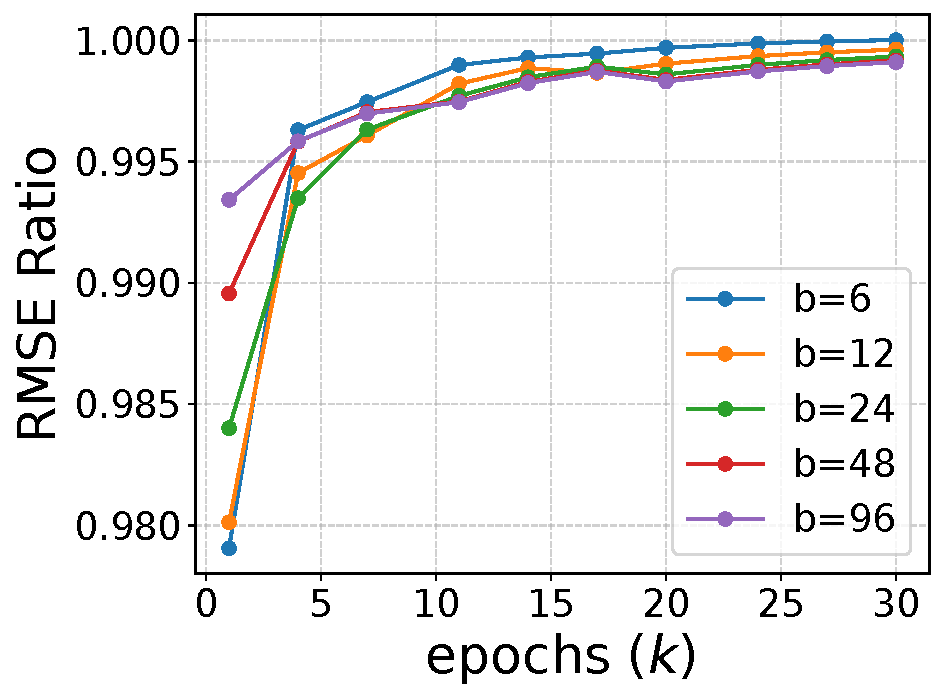
\includegraphics[width=0.4\linewidth]{images/RMSE_normalized_lambda_CGD_ratio.pdf}
    \caption{Ratio of RMSE for column-normalized \method to \method for varying number of epochs $k$ and number of iterations per epoch (separation parameter) $b$. Small $k$  yields a larger improvement from normalization.}
    \label{fig:rmse_normalized_ratio}
\end{figure}
The performance of \method can be further improved by column normalization.
Let
$D = \mathrm{diag}(d_1, \dots, d_n)$
denote the column norms of the matrix $C_\lambda$, and consider the normalized
\method factorization with strategy matrix $C_\lambda D^{-1}$.

It has been observed that column normalization improves performance for banded
matrices \citep{pillutla2025correlated}, and it provably improves both RMSE and
MaxSE for the square-root factorization under single participation
\citep{henzinger2025normalized}. The efficiency of the \method is preserved, in fact any linear noise correlation via matrix $C^{-1}$ can be done without loss of efficiency, we formulate it as the following proposition.

\begin{proposition}[Cost of column normalization]
Let $C\in\mathbb{R}^{n\times n}$ be invertible and let $Z\in\mathbb{R}^n$ be any noise vector.
Let $D=\mathrm{diag}(d_1,\dots,d_n)$ with $d_j>0$ (e.g., $d_j=\|C_{:,j}\|_2$), and define the
column-normalized matrix $\widetilde C \;=\; C D^{-1}$.
Then for any $Z$, $
\widetilde C^{-1} Z \;=\; D\,(C^{-1}Z)$.
Consequently, if computing $C^{-1}Z$ has time complexity $T(n)$, then computing
$\widetilde C^{-1}Z$ has time complexity $T(n)+\mathcal{O}(n)$, i.e., only $\mathcal{O}(1)$
additional work per component (one scaling by $d_i$).
\end{proposition}

\begin{proof}
Since $\widetilde C = C D^{-1}$, we have $\widetilde C^{-1} = D C^{-1}$. Multiplying by $Z$
gives $\widetilde C^{-1}Z = D(C^{-1}Z)$. The extra cost beyond $C^{-1}Z$ is applying the
diagonal matrix $D$, which is $n$ scalar multiplications.
\end{proof}


All efficiency properties are preserved: to correlate the noise $Z$, we first
multiply it by $C_\lambda^{-1}$, which we have shown can be computed
efficiently, and then rescale it by the diagonal matrix $D$.

There is, however, one subtle issue. The matrix $C_\lambda D^{-1}$ is no longer
Toeplitz, and therefore the sensitivity Theorem~\ref{thm:sensitivity} cannot be
applied directly. In this work, we generalize the sensitivity theorem specifically
for the normalized \method in the following theorem.

\begin{restatable}{lemma}{NormalizedSensitivity}
\label{lem:normalized-sensitivity}
The sensitivity of the column-normalized \method with strategy matrix $C_\lambda$ and column norms
$D = \mathrm{diag}(d_1,\dots,d_n)$ is given by
\begin{equation}
    \mathrm{sens}_{k,b}(C_\lambda D^{-1})
    =
    \Big\|
        \sum_{j=0}^{k-1} (C_\lambda D^{-1})_{:,\, jb+1}
    \Big\|_2 .
\end{equation}
\end{restatable}

For the amplified version, there are no such restrictions: the Balls-in-Bins accountant
applies to any positive lower-triangular matrix, which includes the (normalized)
\method matrices. 

We show numerically that the column normalization leads to the improvement in RMSE metric, see Figure \ref{fig:rmse_normalized_ratio}.

\begin{restatable}{lemma}{rmseComparisonLemma}
\label{lem:rmse-comparison}
For any $\lambda \in (0,1)$ under the single-participation model, the RMSE of column-normalized \method is smaller than that of the \method.
\end{restatable}
%\clearpage
\section{Full Experiment Details}


\begin{table}[t]
\centering
\caption{Runtime comparison (seconds) in  across models and bandwidths for CIFAR-10 training over one epoch. CNN, WideResNet-40, and ViT-B/16 are trained using 8 CPU cores and an NVIDIA A100 GPU. We use a batch size of 512 with a physical batch size of 64. For ViT-L/16 we use NVIDIA H100 GPU with 64 cores and physical batch size 16.}
\label{tab:runtime_comparison}
\resizebox{\textwidth}{!}{
\begin{tabular}{lccccccccc}
\hline
 & \multicolumn{3}{c}{\textbf{DP-SGD}} 
 & \multicolumn{3}{c}{\textbf{GPU Noise Regeneration}} 
 & \multicolumn{3}{c}{\textbf{CPU Noise Buffer}} \\
\cline{2-10}
\textbf{Model} 
 &   &   & 
 & 2 & 4 & 16 
 & 2 & 4 & 16 \\
\hline
CNN (0.3M)
 & & $18.9 \pm 0.7$  &  
 & $18.8 \pm 0.7$ & $18.9 \pm 0.5$ & $20.1 \pm 0.8$
 & $18.6 \pm 0.7$ & $18.9 \pm 0.4$ & $19.4 \pm 0.7$ \\
 
WideResNet-40 (9M)
 & & $133.7 \pm 2.2$ & 
 & $133.5 \pm 1.2$ & $136.9 \pm 1.3$ & $144.1 \pm 1.0$
 & $143.5 \pm 2.3$ & $143.1 \pm 1.5$ & $149.6 \pm 1.9$ \\

ViT-B/16 (86M)
 & & $825.3 \pm 1.8$   &  
 & $826.9 \pm 3.2$ & $829.2 \pm 1.7$ & $842.9 \pm 2.8$
 & $886.9 \pm 2.0$ & $897.9 \pm 3.0$ & $987.2 \pm 0.4$ \\

ViT-L/16 (307M)
 & & $1357.9 \pm 1.9$ &
 & $1363.2 \pm 4.2$ & $1364.7 \pm 4.6$ & $1367.3 \pm 2.2$
 & $1507.6 \pm 3.1$ & $1543.3 \pm 6.3$ & $1842.7 \pm 12.9$ \\

ViT-H/14 (632M)
 & & $3252.5 \pm 3.8$ &
 & $3275.7 \pm 6.2$ & $3288.6 \pm 4.6$ & $3290.8 \pm 8.5$
 & $3544.2 \pm 3.1$ & $3598.9 \pm 6.7$ & $4068.9 \pm 7.2$ \\
\hline
\end{tabular}
}
\end{table}

\begin{table}[t]
\centering
\caption{Runtime comparison (seconds) across models and noise-buffer sizes for IMDB fine-tuning over one epoch. We use batch size $128$. LSTM, BERT-Tiny, and BERT-Base are run on an NVIDIA A100 with 64 CPU cores and physical batch size $64$; BERT-Large is run on an NVIDIA H100 with 64 CPU cores with physical batch size $16$.}
\label{tab:runtime_comparison_imdb}
\resizebox{\textwidth}{!}{
\begin{tabular}{lccccccccc}
\hline
 & \multicolumn{3}{c}{\textbf{DP-SGD}} 
 & \multicolumn{3}{c}{\textbf{GPU Noise Regeneration}} 
 & \multicolumn{3}{c}{\textbf{CPU Noise Buffer}} \\
\cline{2-10}
\textbf{Model} 
 &   &   & 
 & 2 & 4 & 16 
 & 2 & 4 & 16 \\
\hline

LSTM (1M)
 & & $310.2 \pm 3.8$ &
 & $317.1 \pm 1.3$ & $317.7 \pm 5.8$ & $318.8 \pm 3.6$
 & $322.4 \pm 3.7$ & $322.8 \pm 3.1$ & $325.9 \pm 3.0$ \\

BERT-Tiny (3M)
 & & $14.6 \pm 0.3$ &
 & $15.8 \pm 0.5$ & $15.6 \pm 0.3$ & $20.8 \pm 0.6$
 & $21.4 \pm 0.4$ & $22.1 \pm 0.3$ & $25.8 \pm 0.4$ \\

BERT-Base (110M)
 & & $334.3 \pm 0.8$ &
 & $339.1 \pm 0.5$ & $342.1 \pm 1.6$ & $369.7 \pm 1.0$
 & $543.3 \pm 3.2$ & $554.4 \pm 4.8$ & $671.7 \pm 4.5$ \\

BERT-Large (340M)
 & & $499.0 \pm 0.1$ &
 & $508.7 \pm 2.0$ & $513.0 \pm 1.5$ & $539.2 \pm 1.7$
 & $846.9 \pm 3.2$ & $859.4 \pm 3.9$ & $1236.5 \pm 17.5$ \\

\hline
\end{tabular}
}
\end{table}

\begin{table}[t]
\caption{Hyperparameters for the experiments in Figure~\ref{fig:method_comparison_cifar_10}, for each privacy budget $\epsilon$: batch size $B$, clipping norm $\zeta$, and method-specific $\lambda$ and learning rate (lr). Hyperparameters are chosen based on performance on the validation set.
}
\centering
\small
\setlength{\tabcolsep}{4pt}
\begin{tabular}{lcccccccccccccc}
\toprule
& & &
\multicolumn{2}{c}{$\epsilon=0.25$}
& \multicolumn{2}{c}{$\epsilon=0.5$}
& \multicolumn{2}{c}{$\epsilon=1$}
& \multicolumn{2}{c}{$\epsilon=2$}
& \multicolumn{2}{c}{$\epsilon=4$}
& \multicolumn{2}{c}{$\epsilon=8$} \\
\cmidrule(lr){4-5}\cmidrule(lr){6-7}\cmidrule(lr){8-9}\cmidrule(lr){10-11}\cmidrule(lr){12-13}\cmidrule(lr){14-15}
Method & $B$ & $\zeta$
& $\lambda$ & lr
& $\lambda$ & lr
& $\lambda$ & lr
& $\lambda$ & lr
& $\lambda$ & lr
& $\lambda$ & lr \\
\midrule
DP-SGD
& 128 & 8
& 0 & 0.05
& 0 & 0.08
& 0 & 0.2
& 0 & 0.2
& 0 & 0.2
& 0 & 0.2 \\

DP-$\lambda$CGD
& 128 & 8
& 0.8  & 0.05
& 0.9  & 0.08
& 0.9  & 0.2
& 0.9  & 0.2
& 0.95 & 0.5
& 0.95 & 0.5 \\

BandInvMF ($p=2$)
& 128 & 8
& 0.977 & 0.02
& 0.977 & 0.05
& 0.977 & 0.08
& 0.977 & 0.2
& 0.977 & 0.2
& 0.977 & 0.5 \\

BandInvMF ($p=16$)
& 128 & 8
& --- & 0.02
& --- & 0.08
& --- & 0.08
& --- & 0.2
& --- & 0.5
& --- & 0.5 \\

BISR ($p=2$)
& 128 & 8
& 0.5 & 0.05
& 0.5 & 0.08
& 0.5 & 0.1
& 0.5 & 0.1
& 0.5 & 0.2
& 0.5 & 0.2 \\

BISR ($p=16$)
& 128 & 8
& --- & 0.05
& --- & 0.1
& --- & 0.2
& --- & 0.2
& --- & 0.5
& --- & 0.5 \\

BLT
& 128 & 8
& --- & 0.05
& --- & 0.1
& --- & 0.2
& --- & 0.5
& --- & 0.5
& --- & 0.5 \\
\bottomrule
\end{tabular}

\label{tab:hyperparams}
\end{table}



\begin{table}[t]
\centering
\caption{RMSE for different mechanisms across privacy budgets $\epsilon$. The first column reports results without amplification by subsampling; in this setting, BandMF \citep{scalingmckenna2024} with full bandwidth achieves the best performance. When Balls-in-Bins amplification via subsampling is applied, other methods perform better, including \method, BLT \citep{dvijotham2024efficient}, and BISR \citep{kalinin2025back} with bandwidth $p=16$. In the high-privacy regime, subsampling substantially affects RMSE, and methods that account for amplification, especially \method, benefit the most.}
\label{tab:eps_all}
\begin{tabular}{lccccccc}
\toprule
Method & $\epsilon=8$ (w/o Amp) & $\epsilon=8$ & $\epsilon=4$ & $\epsilon=2$ & $\epsilon=1$ & $\epsilon=0.5$ & $\epsilon=0.25$ \\
\midrule
BandInvMF ($p=2$)  & 12.69 & 9.70  & 14.90 & 24.41 & 43.66 & 82.77 & 125.87 \\
BandInvMF ($p=4$)  & 10.27 & 8.07  & 12.48 & 20.76 & 37.37 & 70.90 & 130.48 \\
BandInvMF ($p=16$) & 8.54  & 6.56  & 11.23 & 20.17 & 37.09 & 71.08 & 130.90 \\
BandInvMF ($p=64$) & 8.15  & 6.39  & 11.36 & 20.87 & 39.13 & 74.06 & 140.38 \\
BandInvMF ($p=b$)  & 7.87  & 5.66  & 9.86  & 17.76 & 33.25 & 62.84 & 119.20 \\
\addlinespace
BLT & 8.14 & 5.87 & 10.67 & 19.50 & 35.97 & 69.41 & 127.69 \\
\addlinespace
DP-$\lambda$CGD ($\lambda=0.975$) & 12.73 & 9.33  & 14.03 & 21.45 & 36.40 & 68.37 & 125.69 \\
DP-$\lambda$CGD ($\lambda=0.95$)  & 14.74 & 10.27 & 15.28 & 21.45 & 31.70 & 56.75 & 103.44 \\
DP-$\lambda$CGD ($\lambda=0.9$)   & 19.72 & 13.25 & 18.42 & 24.73 & 33.66 & 54.33 & 97.73 \\
\addlinespace
BISR ($p=2$)  & 48.45 & 30.52 & 40.58 & 49.44 & 58.16 & 71.20 & 105.09 \\
BISR ($p=4$)  & 33.47 & 21.00 & 27.97 & 34.87 & 42.50 & 58.27 & 98.52 \\
BISR ($p=16$) & 17.95 & 11.50 & 15.75 & 21.10 & 20.25 & 52.81 & 96.45 \\
BISR ($p=64$) & 10.50 & 6.81  & 9.87  & 15.92 & 28.80 & 53.89 & 101.90 \\
BISR ($p=b$)  & 8.45  & 6.34  & 11.30 & 20.77 & 38.96 & 73.70 & 139.68 \\
\addlinespace
BSR ($p=2$)  & 62.51 & 39.65 & 51.87 & 62.97 & 74.14 & 88.33 & 116.43 \\
BSR ($p=4$)  & 46.80 & 29.29 & 39.32 & 48.13 & 57.03 & 70.47 & 104.90 \\
BSR ($p=16$) & 26.27 & 16.88 & 22.41 & 28.59 & 36.78 & 55.03 & 97.09 \\
BSR ($p=64$) & 14.89 & 9.62  & 13.32 & 18.88 & 29.34 & 52.16 & 97.51 \\
BSR ($p=b$)  & 8.15  & 5.49  & 9.31  & 17.06 & 31.95 & 60.43 & 114.52 \\
\addlinespace
BandMF ($p=2$)  & 59.44 & 37.67 & 49.08 & 59.95 & 71.17 & 86.25 & 114.94 \\
BandMF ($p=4$)  & 42.29 & 27.00 & 36.99 & 45.90 & 55.35 & 68.64 & 104.42 \\
BandMF ($p=16$) & 22.05 & 15.00 & 21.20 & 28.13 & 37.06 & 56.29 & 99.33 \\
BandMF ($p=64$) & 12.58 & 8.77  & 13.25 & 19.76 & 31.40 & 56.07 & 104.68 \\
BandMF ($p=b$)  & 7.77  & 5.84  & 10.42 & 19.16 & 35.94 & 68.02 & 128.79 \\
\addlinespace
DP-SGD & 83.85 & 21.82 & 26.27 & 31.68 & 40.10 & 59.17 & 100.27 \\
\bottomrule
\end{tabular}%
\end{table}

\begin{table}[t]
\caption{Time to generate and correlate the noise at the final ($n$th) iteration and buffer size to produce correlated noise in dimension $d$. For BLT, BSR, and BandMF, regeneration requires replaying from iteration 1, so the last-iteration cost is $nd$. All methods also require correlating noise by summing $p$ vectors of size $d$ ($+pd$ in the runtime).}
\centering
\small
\setlength{\tabcolsep}{4.5pt}
\renewcommand{\arraystretch}{1.15}
\begin{tabular}{lcccc}
\toprule
& \multicolumn{2}{c}{Time per iter. Gen + Corr} & \multicolumn{2}{c}{Buffer size} \\
\cmidrule(lr){2-3}\cmidrule(lr){4-5}
Method & w/o regen. & w/ regen. & w/o regen. & w/ regen. \\
\midrule
DP-SGD     & $d + d$  & $d + d$  & --        & -- \\
\method    & $d + 2d$  & $2d + 2d$ & $d$       & -- \\
BandInvMF  & $d + pd$  & $pd+ pd$ & $(p-1)d$  & -- \\
BISR       & $d+ pd$  & $pd+ pd$ & $(p-1)d$  & -- \\
BLT        & $d+ pd$  & $\textcolor{red}{n}d+ pd$ & $(p-1)d$  & -- \\
BSR        & $d+ pd$  & $\textcolor{red}{n}d+ pd$ & $(p-1)d$  & -- \\
BandMF     & $d+ pd$  & $\textcolor{red}{n}d+ pd$ & $(p-1)d$  & -- \\
\bottomrule
\end{tabular}
\label{tab:noise_time_buffer}
\end{table}

\begin{figure*}[t]
    \centering
    \begin{subfigure}{0.30\linewidth}
        \centering
        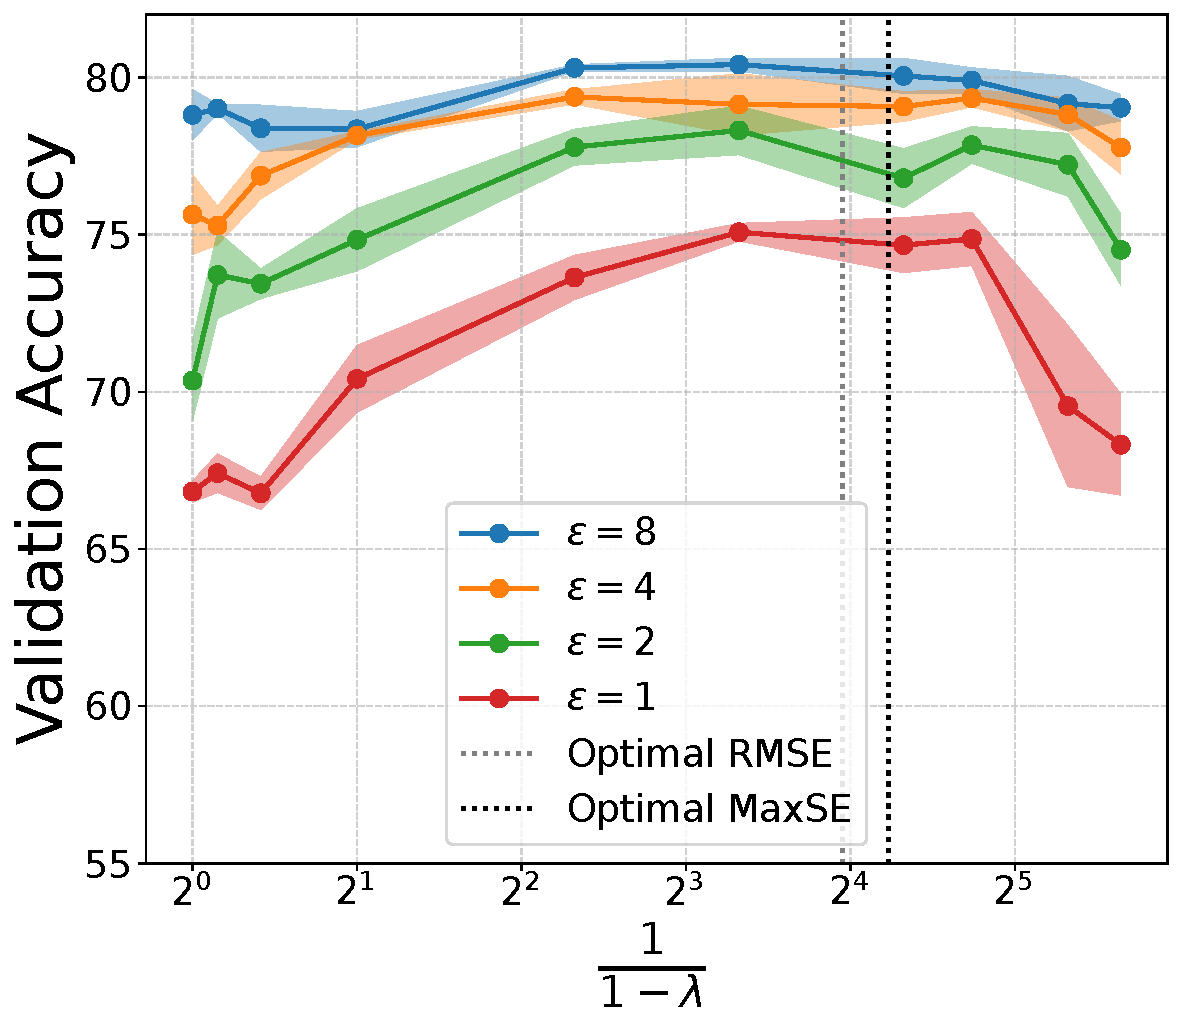
\includegraphics[width=\linewidth]{images/imdb_bandwidth_2_B_512_k_20.pdf}
        \caption{IMDB: $B = 512$, $k=20$}
        \label{fig:imdb128} 
    \end{subfigure}
    \begin{subfigure}{0.30\linewidth}
        \centering
        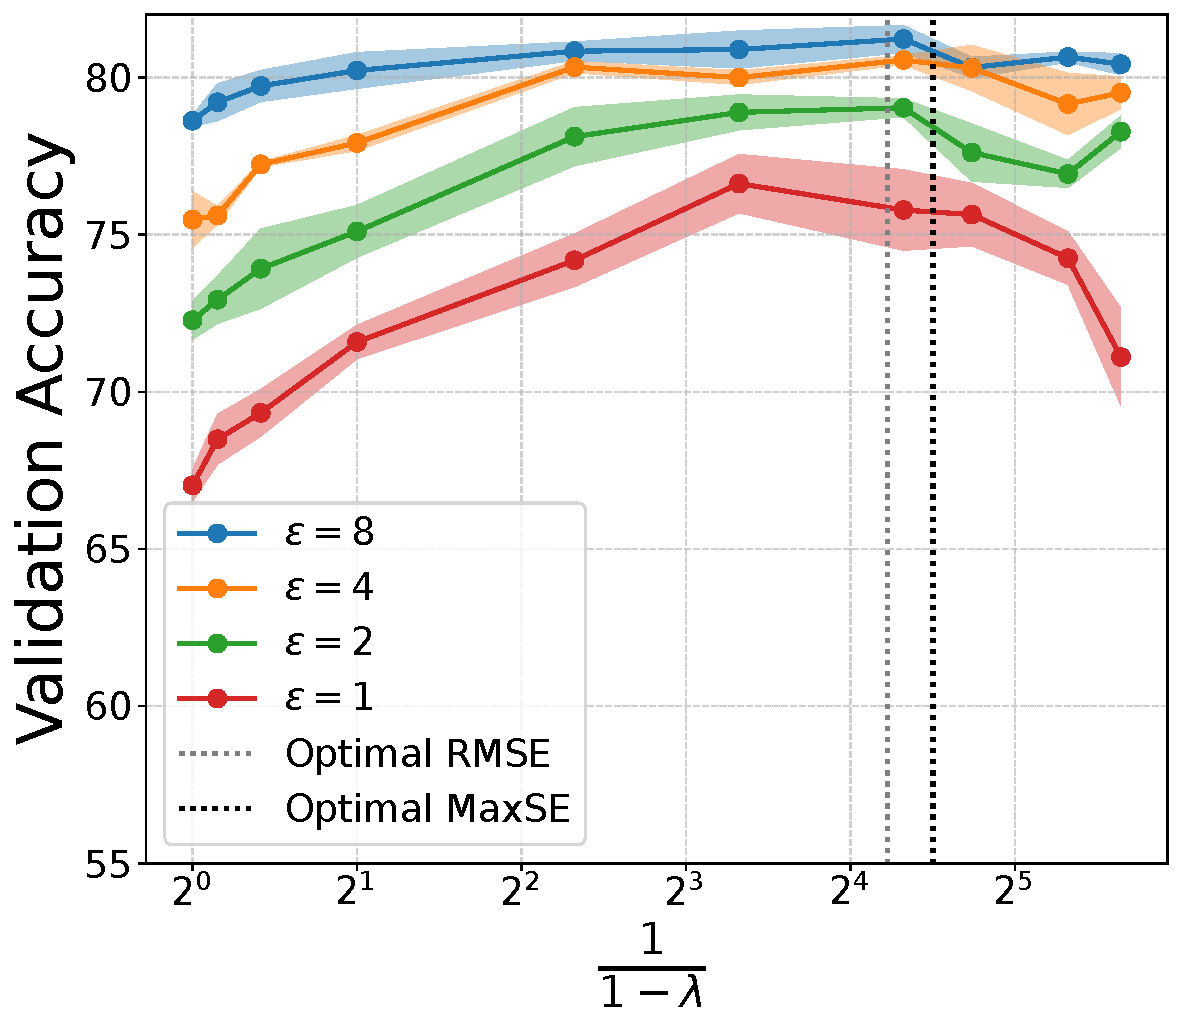
\includegraphics[width=\linewidth]{images/imdb_bandwidth_2_B_512_k_40.pdf}
        \caption{IMDB: $B = 512$, $k=40$}
    \end{subfigure}
    \begin{subfigure}{0.30\linewidth}
        \centering
        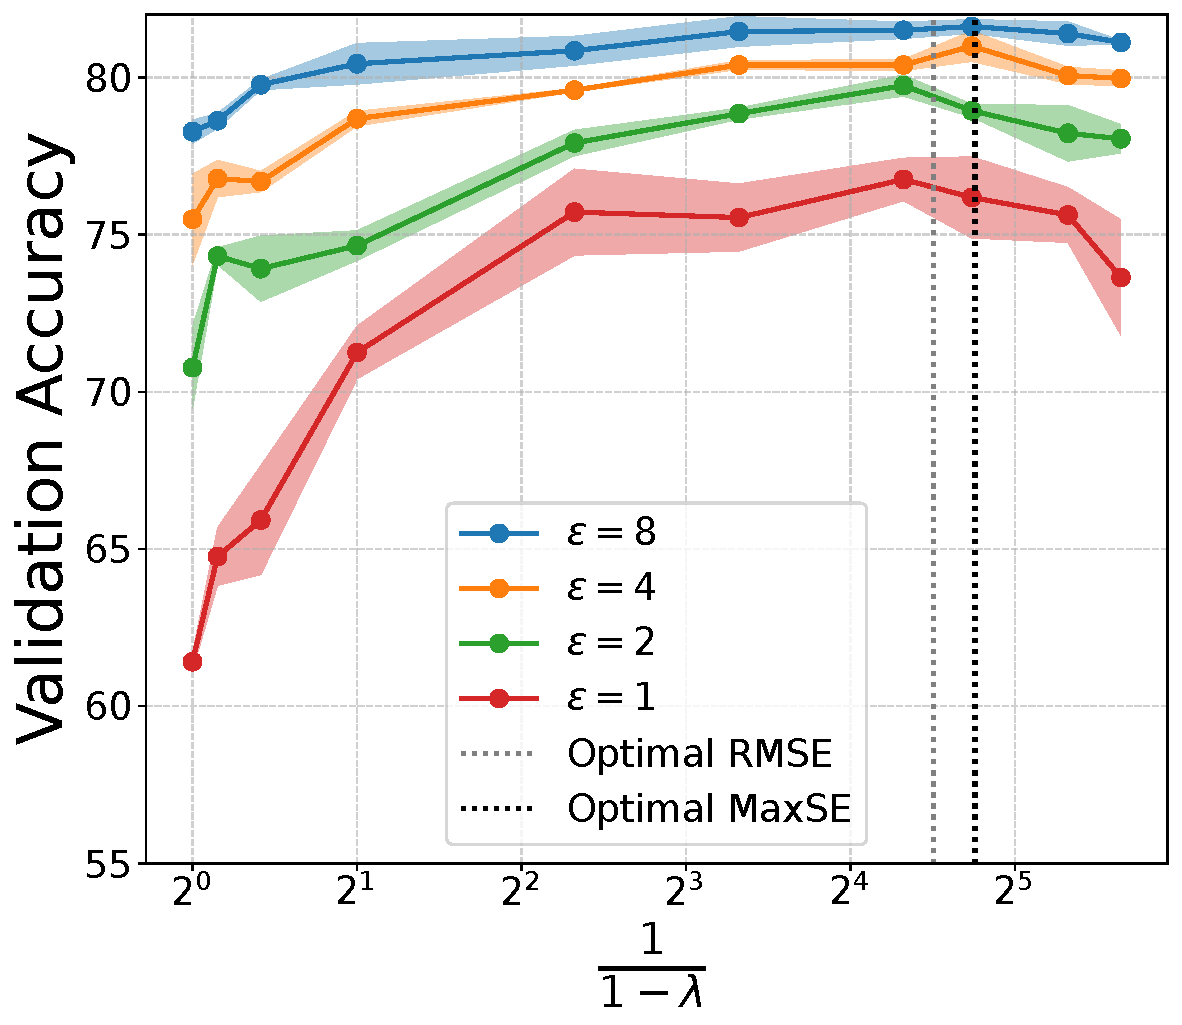
\includegraphics[width=\linewidth]{images/imdb_bandwidth_2_B_512_k_80.pdf}
        \caption{IMDB: $B = 512$, $k=80$}
    \end{subfigure}


    \caption{Validation accuracy with error bars based on three runs for fine-tuning BERT-tiny on the IMDB dataset.  In these runs, we fix the batch size $B$ and the number of iterations per epoch, $b = |D|/B$, and vary the number of epochs $k$. We observe improved utility compared to Figure~\ref{fig:choice_of_lambda}, suggesting that using a larger batch size and training for longer is preferable for overall accuracy. We also find that, in this regime, the optimal mechanism is not DP-SGD. In fact, the trend is the opposite: as the number of epochs increases, the optimal $\lambda$ also increases. This suggests that one can benefit from \method even in long training runs, which are common for DP-SGD. 
   }
    \label{fig:experiments_fixed_batch_size}
\end{figure*}
\clearpage
\begin{figure}[t]
    \centering
    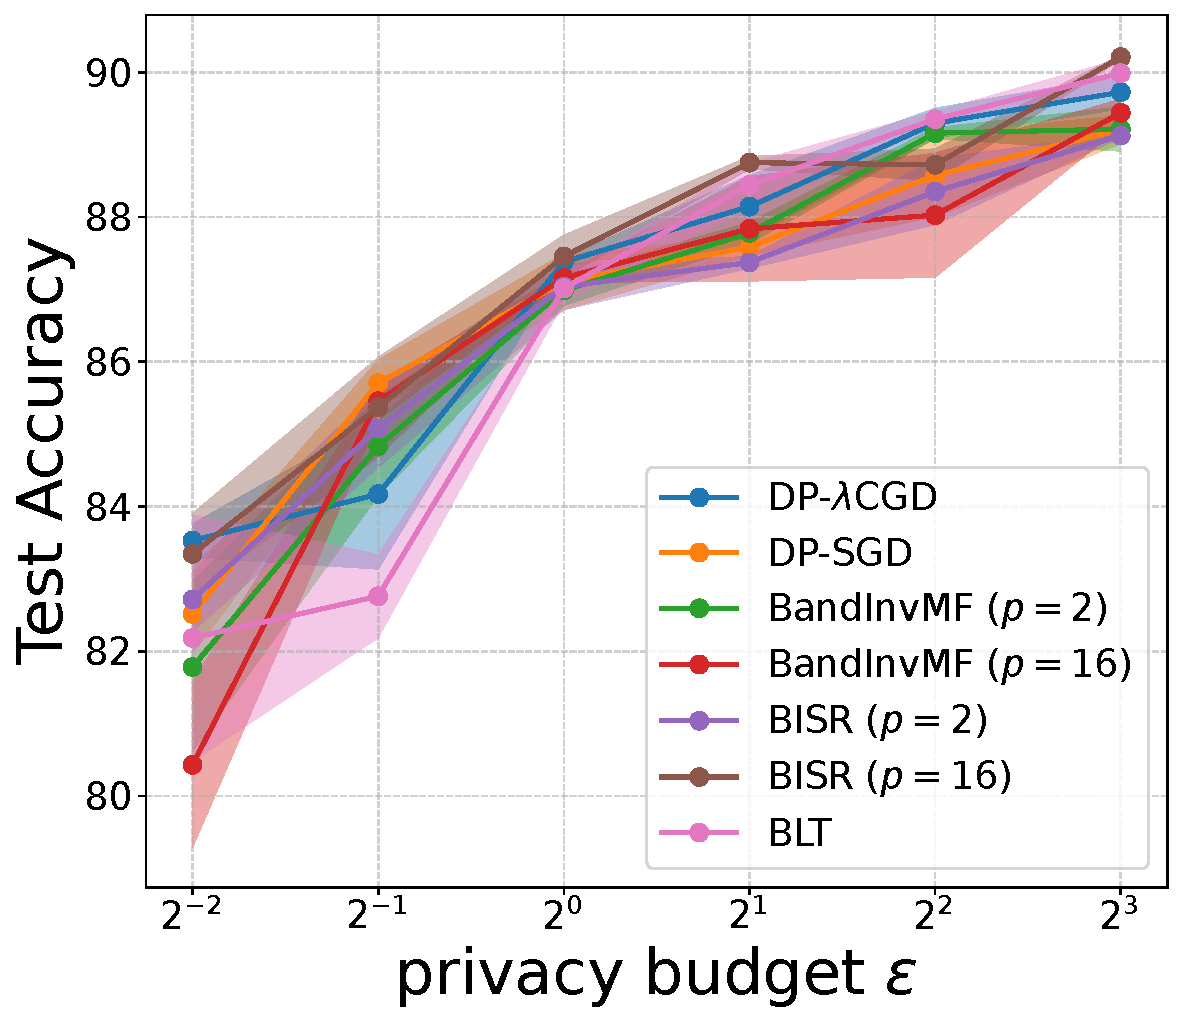
\includegraphics[width=0.4\linewidth]{images/accuracy_vs_epsilon_all_methods_imdb.pdf}
    \caption{Test accuracy of BERT-base (100M) fine-tuned on IMDb for sentiment analysis, trained with batch size $512$ for $10$ epochs. Our proposed \method outperforms DP-SGD at most privacy levels, achieves the best performance under very strict privacy ($\epsilon=1/4$), and performs on par with BLT and BISR factorization.
}
    \label{fig:test_accuracy_imdb}
\end{figure}

\section{Proofs}


\MaxSEBound*
\begin{proof}
First, we compute the squared sensitivity of the matrix $C_{\lambda}$:
\begin{align}
    \mathrm{sens}_{k,b}^2(C_{\lambda})
    &= \left\|\sum\limits_{j = 0}^{k - 1}(C_\lambda)_{:, jb + 1}\right\|_2^2
    = \sum\limits_{j = 0}^{k - 1}\sum\limits_{r = 0}^{b - 1}
      \left(\sum\limits_{m = 0}^{j}\lambda^{jb + r - mb}\right)^2  \\
    &= \sum\limits_{j = 0}^{k - 1}\sum\limits_{r = 0}^{b - 1}
      \lambda^{2r} \left(\frac{1 - \lambda^{b(j + 1)}}{1 - \lambda^b}\right)^2
     = \frac{1 - \lambda^{2b}}{(1- \lambda^2)(1 - \lambda^b)^2}\sum\limits_{j = 1}^{k}(1 - \lambda^{bj})^2.
\end{align}

The squared maximum row $\ell_2$-norm of the matrix $AC_{\lambda}^{-1}$ is
\begin{equation}
    \|AC_{\lambda}^{-1}\|_{2\to \infty}^2 = 1 + (1 - \lambda)^2(n - 1).
\end{equation}

Combining these expressions gives the squared maximum error. To prove the claimed bound, we consider two regimes.

First, suppose $k \ge \sqrt{n}$ and set $\lambda = e^{-1/b}$. This yields
\begin{align}
    \|AC_{\lambda}^{-1}\|_{2\to \infty}^2 \cdot \mathrm{sens}_{k,b}^2(C_{\lambda}) &= \left(1 + \frac{n - 1}{b^2} + O(nb^{-4})\right) \left(\frac{1 - e^{-2}}{(2b^{-1} + O(b^{-2}))(1 - e^{-1})^2} (k + O(1))\right)\\
    &= O\left(\frac{nkb}{b^2}\right) = O(k^2),
\end{align}
assuming $n=kb$.

If $k < \sqrt{n}$, take $\lambda = e^{-1/\sqrt{n}}$. Then $\lambda^b = e^{-\sqrt{n}/k} < 1/e = O(1)$ and $1 -\lambda^{b} = \Theta(1)$, then
\begin{equation}
    \|AC_{\lambda}^{-1}\|_{2\to \infty}^2 \cdot \mathrm{sens}_{k,b}^2(C_{\lambda}) = O(1) \left(\frac{O(1)}{2/\sqrt{n} + O(1/n)}O(k)\right) = O(k\sqrt{n}).
\end{equation}

Combining the two bounds and taking square roots yields the claimed upper bound.
\end{proof}


\MaxSEvsRMSEMinimizerInequality*
\begin{proof}
Define, for $\gamma>0$,
\begin{equation}
    F_{\gamma}(\lambda) = \bigl(1 + (1-\lambda)^2 (n-1)\gamma\bigr)\,\mathrm{sens}^2(C_{\lambda}).
\end{equation}
Then squared MaxSE is given by $F_1(\lambda)$ and squared MeanSE is given by $F_{1/2}(\lambda)$.
We claim that $\frac{F_1(\lambda)}{F_{1/2}(\lambda)}$ is a monotonically decreasing function of $\lambda$.
Indeed, for $\lambda\in(0,1)$:
\begin{equation}
\frac{d}{d\lambda}\left(\frac{F_1(\lambda)}{F_{1/2}(\lambda)}\right)
= \frac{d}{d\lambda}\left(\frac{1 + (1-\lambda)^2(n-1)}{1 + (1-\lambda)^2(n-1)/2}\right)
= -\frac{(n-1)(1-\lambda)}{\left(1+(1-\lambda)^2(n-1)/2\right)^2} < 0.
\end{equation}

Let $\lambda_1$ be a minimizer of $F_1(\lambda)$ and let $\lambda_{1/2}$ be a minimizer of $F_{1/2}(\lambda)$.
Assume for contradiction that $\lambda_1 < \lambda_{1/2}$.
Since $\lambda_1$ and $\lambda_{1/2}$ are minimizers and $\mathrm{sens}(C_{\lambda})>0$, we have
\begin{equation}
    F_{1}(\lambda_{1}) \le F_1(\lambda_{1/2})
    \quad\text{and}\quad
    F_{1/2}(\lambda_{1/2}) \le F_{1/2}(\lambda_{1}).
\end{equation}
Combining these two inequalities gives 
\begin{equation}
    \frac{F_{1}(\lambda_{1})}{F_{1/2}(\lambda_{1})}
    \le
    \frac{F_{1}(\lambda_{1/2})}{F_{1/2}(\lambda_{1/2})}.
\end{equation}
However, the ratio $\frac{F_1(\lambda)}{F_{1/2}(\lambda)}$ is decreasing in $\lambda$, and $\lambda_1 < \lambda_{1/2}$ would imply the reverse inequality, which is a contradiction.
Therefore $\lambda_1 \ge \lambda_{1/2}$.
\end{proof}


\begin{lemma}
\begin{equation}
    \inf_{BC=A}\frac{1}{\sqrt{n}}\|B\|_F \cdot \mathrm{sens}_{n,1}(C)
    \;\ge\;
    \inf_{BC=A}\frac{1}{\sqrt{n}}\|B\|_F \|Ce\|_2
    \;=\;
    \frac{1}{\sqrt{n}}\|Ae\|_2
    \;=\;
    \sqrt{\frac{(n+1)(2n+1)}{6}}.
\end{equation}
\end{lemma}

\begin{proof}

We first consider the sensitivity. By definition,
\begin{equation}
    \mathrm{sens}_{n,1}(C)
    = \sup_{X \sim X'} \|CX - CX'\|_F,
\end{equation}
where neighboring datasets may differ in any coordinates and each
$X_i, X'_i$ has $\ell_2$-norm at most $1$.
To obtain a lower bound, take $X$ and $X'$ that differ in all coordinates
and lie along a single dimension. Then $\|C(X-X')\|_F = \|Ce\|_2$. This gives the first inequality.

Next, for any factorization $A = BC$,
\begin{equation}
    \|Ae\|_2
    = \|BCe\|_2
    \le \|B\|_2 \|Ce\|_2
    \le \|B\|_F \|Ce\|_2.
\end{equation}
Thus
\begin{equation}
    \frac{1}{\sqrt{n}}\|B\|_F \|Ce\|_2
    \ge \frac{1}{\sqrt{n}}\|Ae\|_2.
\end{equation}

To show this bound is tight, we construct factorizations approaching equality.
Let $R$ be a rotation such that $RAe = \|Ae\|_2\, e_1$. For $\lambda > 0$, define $D_\lambda = \mathrm{diag}(1, \lambda, \ldots, \lambda)$,
and set
\begin{equation}
    C_\lambda = D_\lambda^{-1} R A,
    \qquad
    B_\lambda = R^{-1} D_\lambda  = R^{T}D_\lambda.
\end{equation}
Then
\begin{equation}
    \|C_\lambda e\|_2
    = \|D_\lambda^{-1} R Ae\|_2
    = \|D_\lambda^{-1} e_1\|_2 \cdot \|Ae\|_2
    = \|Ae\|_2,
\end{equation}
and
\begin{equation}
    \|B_\lambda\|_F
    = \|R^{T} D_\lambda \|_F
    = \|D_\lambda\|_F
    = \sqrt{1 + \lambda^2 (n-1)}.
\end{equation}
As $\lambda \to 0$, we have $\|B_\lambda\|_F \to 1$, so $\|B_\lambda\|_F \|C_\lambda e\|_2 \to \|Ae\|_2$,
proving the infimum equals $\|Ae\|_2$.

Finally, since $Ae = (1,2,\ldots,n)^T$,
\begin{equation}
    \|Ae\|_2
    = \sqrt{\sum_{j=1}^n j^2}
    = \sqrt{\frac{n(n+1)(2n+1)}{6}}.
\end{equation}

\end{proof}


\begin{lemma}
\begin{equation}
    \inf_{BC=A}\frac{1}{\sqrt{n}}\|B\|_F \cdot \mathrm{sens}_{n,1}(C)
    \;\le\;
    \inf_{\substack{BC=A \\ C \ge 0}}
        \frac{1}{\sqrt{n}}\|B\|_F \|Ce\|_2
    \;\le\;
    \frac{1}{\sqrt{n}} \sum_{j=1}^{n} \sqrt{j}
    \;\sim\;
    \frac{2n}{3}.
\end{equation}
\end{lemma}

\begin{proof}

The first inequality was proved in \citet{choquette2023amplified} (see Proposition E.1) under the stronger condition $C^T C \ge 0$.  
When $C \ge 0$, the sensitivity can be computed as the supremum over all participation patterns of the corresponding $\ell_2$ norm. In this case,
\begin{equation}
    \mathrm{sens}_{n,1}(C) = \|Ce\|_2,
\end{equation}
which yields the inequality.

For the second inequality, consider the following diagonal factorization:
\begin{equation}
    C = \mathrm{diag}\bigl(n^{1/4}, (n-1)^{1/4}, \ldots, 1^{1/4}\bigr),
    \qquad
    B_{i,j} = 
    \begin{cases}
        (n - j + 1)^{-1/4}, & i \ge j,\\[3pt]
        0, & \text{otherwise}.
    \end{cases}
\end{equation}

Then
\begin{equation}
    \|Ce\|_2 
    = \sqrt{\sum_{j=1}^{n} \sqrt{j}}, \quad
    \|B\|_F
    = \sqrt{
        \sum_{j=1}^{n} 
        (n - j + 1) \cdot (n - j + 1)^{-1/2}
    }
    =
    \sqrt{\sum_{j=1}^{n} \sqrt{j}}.
\end{equation}

Thus
\begin{equation}
    \frac{1}{\sqrt{n}} \, \|B\|_F \|Ce\|_2
    = 
    \frac{1}{\sqrt{n}} \sum_{j=1}^{n} \sqrt{j},
\end{equation}
giving the stated upper bound. Finally, by Cauchy--Schwarz inequality, this diagonal factorization is optimal among all diagonal choices of $C$.
\end{proof}



\NormalizedSensitivity*

\begin{proof}
We first note that the matrix $C_\lambda D^{-1}$ is no longer Toeplitz, and therefore Theorem~\ref{thm:sensitivity} does not apply directly. We instead repeat the argument of the proof of that theorem for this specific matrix.

For an element-wise nonnegative matrix $C$, the sensitivity can be written \citep{choquette2023amplified} as
\begin{equation}
    \mathrm{sens}(C)
    = \sup_{\pi} \sqrt{\sum_{i,j \in \pi} \langle C_{:,i}, C_{:,j} \rangle},
\end{equation}
where $\pi$ ranges over sets of at most $k$ column indices with minimum separation $b$.

Following the argument of \citet{kalinin2024}, we show that the maximizing set $\pi$ consists of the leftmost admissible columns. Specifically, if the optimal indices are not the leftmost ones (subject to $b$-separation), then the entire block can be shifted left without decreasing the objective. It suffices to show two facts:
\begin{enumerate}
    \item If $i+b<j$, then
    \[
        \langle (C_\lambda D^{-1})_{:,i}, (C_\lambda D^{-1})_{:,j} \rangle
        \le
        \langle (C_\lambda D^{-1})_{:,i}, (C_\lambda D^{-1})_{:,j-1} \rangle .
    \]
    \item If $i>1$ and $i+b \le j$, then
    \[
        \langle (C_\lambda D^{-1})_{:,i}, (C_\lambda D^{-1})_{:,j} \rangle
        \le
        \langle (C_\lambda D^{-1})_{:,i-1}, (C_\lambda D^{-1})_{:,j-1} \rangle .
    \]
\end{enumerate}
Since all columns are normalized to unit norm, these properties imply that the maximum sensitivity is attained by choosing the leftmost $k$ columns with separation $b$, i.e., indices $\{1,\, 1+b,\, \dots,\, 1+(k-1)b\}$.

We now verify the two claims. The inner product between the $i$th and $j$th columns of $C_\lambda D^{-1}$ is
\begin{equation}
    \langle (C_\lambda D^{-1})_{:,i}, (C_\lambda D^{-1})_{:,j} \rangle
    =
    \frac{1}{d_i d_j}
    \sum_{t=0}^{n-j} \lambda^{t} \lambda^{j-i+t},
\end{equation}
where
\begin{equation}
    d_i
    = \sqrt{\sum_{t=0}^{n-i} \lambda^{2t}}
    = \sqrt{\frac{1-\lambda^{2(n-i+1)}}{1-\lambda^2}} .
\end{equation}

Similarly, the inner product between columns $i$ and $j-1$ is
\begin{equation}
    \langle (C_\lambda D^{-1})_{:,i}, (C_\lambda D^{-1})_{:,j-1} \rangle
    =
    \frac{1}{d_i d_{j-1}}
    \sum_{t=0}^{n-j+1} \lambda^{t} \lambda^{j-i-1+t}.
\end{equation}
Taking the difference yields
\begin{align}
    &\langle (C_\lambda D^{-1})_{:,i}, (C_\lambda D^{-1})_{:,j-1} - (C_\lambda D^{-1})_{:,j} \rangle \\
    &\qquad
    = \frac{\lambda^{j-i-1}}{d_i d_{j-1}} d_{j-1}^2
      - \frac{\lambda^{j-i}}{d_i d_j} d_j^2
    = \frac{\lambda^{j-i-1}}{d_i} (d_{j-1} - \lambda d_j) \ge 0,
\end{align}
since the sequence $(d_j)$ is decreasing. This proves the first claim.

For the second claim, we consider
\begin{align}
    &\langle (C_\lambda D^{-1})_{:,i-1}, (C_\lambda D^{-1})_{:,j-1} \rangle
    - \langle (C_\lambda D^{-1})_{:,i}, (C_\lambda D^{-1})_{:,j} \rangle \\
    &\qquad
    = \lambda^{j-i}
    \left(
        \frac{d_{j-1}}{d_{i-1}} - \frac{d_j}{d_i}
    \right).
\end{align}
Thus it suffices to show that
\[
    \frac{d_{j-1} d_i}{d_{i-1} d_j} \ge 1.
\]
Using the explicit form of $d_i$, we obtain
\begin{equation}
    \frac{d_{j-1} d_i}{d_{i-1} d_j}
    =
    \sqrt{
        \frac{
            (1-\lambda^{2(n-j+2)})(1-\lambda^{2(n-i+1)})
        }{
            (1-\lambda^{2(n-i+2)})(1-\lambda^{2(n-j+1)})
        }
    }.
\end{equation}
Expanding the numerator and denominator, we see that this ratio is at least one if and only if
\begin{equation}
    \lambda^{2(n - j + 1)} + \lambda^{2(n - i + 2)}
    -
     \lambda^{2(n - j + 2)} - \lambda^{2(n - i + 1)}
    \ge 0.
\end{equation}
Rearranging terms gives
\begin{equation}
    (1 - \lambda^2)
    \bigl(
        \lambda^{2(n - j + 1)} - \lambda^{2(n - i + 1)}
    \bigr)
    \ge 0,
\end{equation}
which holds whenever $i \le j$. This concludes the proof.
\end{proof}


\rmseComparisonLemma*

\begin{proof}
The strategy matrix of \method is
\begin{equation}
    C_{\lambda} = \begin{pmatrix}
        1 & 0 & \cdots &0\\
        \lambda & 1 & \cdots & 0\\
        \vdots & \vdots & \ddots & \vdots\\
        \lambda^{n - 1} & \lambda^{n - 2} & \cdots & 1
    \end{pmatrix}.
\end{equation}

The squared norms of its columns are
\begin{equation}
    d_j^2 = \sum\limits_{i = 0}^{n - j} \lambda^{2i}
    = \frac{1 - \lambda^{2(n - j + 1)}}{1 -\lambda^2}. 
\end{equation}

The sensitivity of $C_{\lambda}$ under single participation is $d_1$.
For the factorization $A = B_{\lambda} C_{\lambda}$, where $A$ is the prefix-sum matrix, the corresponding left matrix is
\begin{equation}
    B_{\lambda} = \begin{pmatrix}
        1 & 0 & 0 & \cdots & 0\\
        1- \lambda & 1 & 0 & \dots &0\\
        1 - \lambda & 1- \lambda & 1 &\cdots & 0\\
        \vdots & \vdots & \vdots & \ddots & \vdots\\
        1 - \lambda & 1- \lambda & 1 - \lambda & \cdots & 1
    \end{pmatrix}.
\end{equation}

Its Frobenius norm can be written as
\begin{equation}
    \|B_{\lambda}\|_{F}^2 = (1 - \lambda)^2 \frac{(n - 1)n}{2} + n.
\end{equation}

The sensitivity of the normalized \method is equal to $1$ by construction.
The normalized strategy matrix is $\tilde{C}_{\lambda} = C_{\lambda} D^{-1}$, and the corresponding left matrix is
$\tilde{B}_{\lambda} = A D C_{\lambda}^{-1}$.
Its entries are
\begin{equation}
    (\tilde{B}_{\lambda})_{i,j} = \begin{cases}
        d_{j} - \lambda d_{j + 1} \quad & \text{if} \quad j < i,\\
        d_j \quad &\text{if} \quad j = i,\\
        0 \quad &\text{otherwise.}
    \end{cases}
\end{equation}
Therefore, its Frobenius norm satisfies
\begin{equation}
    \|\tilde{B}_{\lambda}\|_F^2
    = \sum\limits_{j = 1}^{n} d_j^2
    + \sum\limits_{j = 1}^{n - 1} (d_j - \lambda d_{j + 1})^2 (n - j).
\end{equation}

To show that the normalized \method has lower RMSE than \method, it is sufficient to prove
\begin{equation}
\label{ineq:rmse_norm_method}
    \sum\limits_{j = 1}^{n} d_j^2
    + \sum\limits_{j = 1}^{n - 1} (d_j - \lambda d_{j + 1})^2 (n - j)
    \le d_1^2 \left(n + (1 - \lambda)^2 \frac{(n - 1)n}{2}\right).
\end{equation}

First, we compute the sum of $d_j^2$:
\begin{equation}
\label{eq:d_j_squared_sum}
    \sum\limits_{j = 1}^{n} d_j^2
    = \sum\limits_{j = 1}^{n}\sum\limits_{i = 0}^{n - j }\lambda^{2i}
    = \sum\limits_{i = 0}^{n - 1}\lambda^{2i} (n - i)
    = n d_1^2 - \sum\limits_{j = 1}^{n - 1} j\lambda^{2j}.
\end{equation}

Next, we bound $d_j - \lambda d_{j + 1}$ as follows:
\begin{equation}
\begin{aligned}
    (d_j - \lambda d_{j + 1})^2
    &= d_j^2 +\lambda^2 d_{j + 1}^2 - 2\lambda d_j d_{j + 1}\\
    &= d_{j + 1}^2 + \lambda^{2(n - j)} +\lambda^2 d_{j + 1}^2 -2\lambda d_j d_{j + 1}\\
    &\le (1 -\lambda)^2 d_{j + 1}^2 + \lambda^{2(n - j)}.
\end{aligned}
\end{equation}

Thus,
\begin{align}
    \sum\limits_{j = 1}^{n - 1}(d_j - \lambda d_{j + 1})^2 (n - j)
    &\le (1-\lambda)^2 \sum\limits_{j = 1}^{n -1} d_{j + 1}^2 (n -j)
      + \sum\limits_{j = 1}^{n - 1} j \lambda^{2j} \\
    &\le d_1^2 (1 - \lambda)^2 \sum\limits_{j = 1}^{n - 1} (n- j)
      + \sum\limits_{j = 1}^{n - 1} j \lambda^{2j}\\
    &= d_1^2 (1 - \lambda)^2 \frac{n ( n - 1)}{2 }
      + \sum\limits_{j = 1}^{n - 1} j \lambda^{2j}.
\end{align}

Combining this bound with \eqref{eq:d_j_squared_sum} yields \eqref{ineq:rmse_norm_method}.
\end{proof}



\end{document}

% This document was modified from the file originally made available by
% Pat Langley and Andrea Danyluk for ICML-2K. This version was created
% by Iain Murray in 2018, and modified by Alexandre Bouchard in
% 2019 and 2021 and by Csaba Szepesvari, Gang Niu and Sivan Sabato in 2022.
% Modified again in 2023 and 2024 by Sivan Sabato and Jonathan Scarlett.
% Previous contributors include Dan Roy, Lise Getoor and Tobias
% Scheffer, which was slightly modified from the 2010 version by
% Thorsten Joachims & Johannes Fuernkranz, slightly modified from the
% 2009 version by Kiri Wagstaff and Sam Roweis's 2008 version, which is
% slightly modified from Prasad Tadepalli's 2007 version which is a
% lightly changed version of the previous year's version by Andrew
% Moore, which was in turn edited from those of Kristian Kersting and
% Codrina Lauth. Alex Smola contributed to the algorithmic style files.
